\باب{مخلوط تحلیل تفاعل اور نظریہ مخفی قوہ}\شناخت{باب_مخلوط_تفاعل_اور_نظریہ_مخفی_قوہ}
مساوات لاپلاس \عددی{\nabla^{\,2}u=0} انجینئری حساب میں اہم ترین جزوی تفرقی مساوات میں سے ایک ہے چونکہ  یہ ثقلی میدان (حصہ \حوالہ{حصہ_الاحصاء_ڈھلوان})، ساکن برقی میدان  (حصہ \حوالہ{حصہ_جزوی_مخفی_قوہ})، برقرار حال ایصال حرارت (حصہ \حوالہ{حصہ_نقش_دیگر_تفاعل})، داب نا پذیر بہاو سیال، وغیرہ کے مسئلوں میں پایا جاتا ہے۔ اس مساوات کے حل کو \اصطلاح{نظریہ مخفی قوہ}\فرہنگ{مخفی قوہ!نظریہ}\حاشیہب{potential theory}\فرہنگ{potential!theory} کہتے ہیں۔

دو بعدی صورت جہاں \عددی{u} کارتیسی محدد کے دو محور \عددی{x} اور \عددی{y} کے تابع ہو میں لاپلاس مساوات درج ذیل صورت اختیار کرتی ہے۔
\begin{align*}
\nabla^{\,2}u=u_{xx}+u_{yy}=0
\end{align*}
ہم جانتے ہیں کہ تب اس کے حل مخلوط تحلیلی تفاعل (حصہ \حوالہ{حصہ_تحلیلی_کوشی_ریمان_مساوات_لاپلاس}) کے ساتھ گہرا تعلق رکھتے\حاشیہد{تین بعدی صورت میں ایسا گہرا تعلق نہیں پایا جاتا ہے۔} ہیں۔ ہم اس تعلق پر اب تفصیلاً غور کرتے ہیں اور ماقوا حرکیات اور برقی سکون سے چند مثال بھی پیش کریں گے۔ ہم آگے دیکھیں گے کہ تحلیلی تفاعل کے نتائج کو استعمال کرتے ہوئے ہارمونی تفاعل کی مختلف عمومی خواص  بیان کی جا سکتی ہیں (حصہ \حوالہ{حصہ_مخفی_ہارمونی_تفاعل_عمومی_خواص})۔ آخر میں ہم دائری قرص پر مساوات لاپلاس کے سرحدی مسائل کے حل کا ایک اہم عمومی کلیہ (پوسوں تکملی کلیہ) اخذ کریں گے۔

%===========================
\حصہ{ساکن برقی سکون}
بار بردار ذرات کے مابین قوت کشش یا دفع کو کلیہ کولمب سے حاصل  کیا جا سکتا ہے۔یہ قوت تفاعل \عددی{u} جس کو \اصطلاح{برقی ساکن مخفی قوہ}\فرہنگ{مخفی قوہ!برقی سکونیات}\حاشیہب{electrostatic potential}\فرہنگ{potential!electrostatic} کہتے ہیں کی ڈھلوان ہے، اور بار سے پاک نقطوں پر \عددی{u} مساوات لاپلاس (حصہ \حوالہ{حصہ_جزوی_مخفی_قوہ})
\begin{align*}
\nabla^{\,2}u=0
\end{align*}
کو مطمئن کرتا ہے۔ سطحیں \عددی{u=\text{مستقل}} کو \اصطلاح{ہم قوہ سطحیں}\فرہنگ{ہم قوہ سطحیں}\حاشیہب{equipotential surfaces}\فرہنگ{equipotential!surfaces} کہتے ہیں۔ہر نقطہ \عددی{N} پر \عددی{u} کی ڈھلوان نقطہ \عددی{N} پر سطح \عددی{u=\text{مستقل}} کی قائمہ ہو گی، یعنی برقی قوت اور ہم قوہ سطح آپس میں قائمہ ہوں گے۔

%===================
\ابتدا{مثال}\شناخت{مثال_مخفی_قوہ_متوازی_چادر}\quad \موٹا{متوازی چادروں کے درمیان خطہ میں مخفی قوہ}\\
دو لامتناہی وسعت کی متوازی موصل چادر جنہیں بالترتیب \عددی{U_1} اور \عددی{U_2} برقی دباو پر رکھا گیا ہے کے درمیان مخفی قوہ تلاش کریں (شکل \حوالہ{شکل_مثال_مخفی_قوہ_متوازی_چادر}-الف)۔چادروں کی شکل سے ظاہر ہے کہ \عددی{u} صرف \عددی{x} کا تابع ہو گا لہٰذا مساوات لاپلاس \عددی{u''=0} صورت اختیار کرتی ہے۔دو مرتبہ تکمل لے کر \عددی{u=ax+b} حاصل ہوتا ہے جہاں مستقل \عددی{a} اور \عددی{b} کو چادروں پر برقی دباو \عددی{u} کی سرحدی شرائط سے حاصل کیا جاتا ہے۔مثال کے طور پر اگر چادر \عددی{x=-1} اور \عددی{x=1} پر واقع ہوں تب حل
\begin{align*}
u(x)=\frac{1}{2}(U_2-U_1)x+\frac{1}{2}(U_2+U_1)
\end{align*}
ہو گا۔ہم قوہ سطحیں چادروں کے متوازی سطحیں ہوں گی۔
\begin{figure}
\centering
\begin{subfigure}{0.5\textwidth}
\centering
\begin{tikzpicture}
\pgfmathsetmacro{\klen}{0.25}
\fill[gray!20!white](-2*\klen,-1.5) rectangle (2*\klen,1.5);
\draw(-1,0)--(1,0)node[right]{$x$};
\draw(0,-1.5)--(0,2)node[left]{$y$};
\draw[thick](-2*\klen,-1.5)--(-2*\klen,1.5);
\draw[thick](2*\klen,-1.5)--(2*\klen,1.5);
\draw[](-\klen,-1.5)--(-\klen,1.5);
\draw[](\klen,-1.5)--(\klen,1.5);
\draw[](0,0)node[ocirc]{};
\end{tikzpicture}
\caption*{(الف) متوازی چادروں کے درمیان مخفی قوہ}
\end{subfigure}%
\begin{subfigure}{0.5\textwidth}
\centering
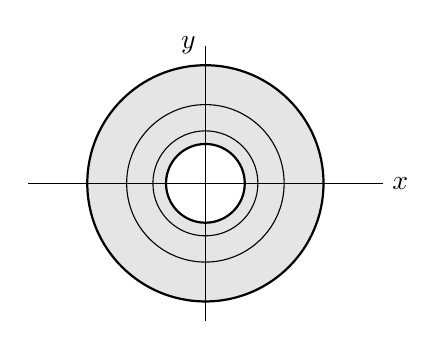
\begin{tikzpicture}
\fill[gray!20!white](0,0) circle (1.5);
\fill[white](0,0) circle (0.5);
\draw(-2.25,0)--(2.25,0)node[right]{$x$};
\draw(0,-1.75)--(0,1.75)node[left]{$y$};
\draw[thick](0,0) circle (0.5);
\draw[thick](0,0)circle (1.5);
\draw(0,0) circle (1);
\draw(0,0) circle (2/3);
\end{tikzpicture}
\caption*{(ب) ہم محور موصل نلکیوں کے درمیان مخفی قوہ}
\end{subfigure}%
\caption{اشکال برائے مثال \حوالہ{مثال_مخفی_قوہ_متوازی_چادر} اور مثال \حوالہ{مثال_مخفی_قوہ_ہم_محوری_نلکی}}
\label{شکل_مثال_مخفی_قوہ_متوازی_چادر}
\end{figure}
\انتہا{مثال}
%=========================
\ابتدا{مثال}\شناخت{مثال_مخفی_قوہ_ہم_محوری_نلکی}\quad \موٹا{ہم محور نلکیوں کے درمیان خطہ میں مخفی قوہ}\\
دو لامتناہی لمبائی کی ہم محور موصل نلکیاں  جنہیں بالترتیب \عددی{U_1} اور \عددی{U_2} مخفی قوہ پر رکھا گیا ہو  کے درمیان مخفی قوہ تلاش کریں (شکل \حوالہ{شکل_مثال_مخفی_قوہ_متوازی_چادر}-ب)۔ یہاں  تشاکل کی بنا \عددی{u} صرف \عددی{r=\sqrt{x^2+y^2}} کا تابع ہو گا اور مساوات لاپلاس
\begin{align*}
ru''+u'=0\quad \quad \text{\RL{(مساوات \حوالہ{مساوات_جزوی_لاپلاسی__رکن_ت} دیکھیں)}}
\end{align*}
صورت اختیار کرتی ہے۔علیحدگی متغیرات کے بعد تکمل لینے سے
\begin{align*}
\frac{u''}{u'}=-\frac{1}{r},\quad \ln u'=-\ln r+\tilde{a},\quad u'=\frac{a}{r},\quad u=a\ln r+b
\end{align*}
حاصل ہو گا جہاں مستقل \عددی{a} اور \عددی{b} کو ہم محوری نلکیوں پر \عددی{u} کی دی گئی قیمتوں سے حاصل کیا جائے گا۔اگرچہ لامتناہی لمبائی کی موصل نلکی کہیں نہیں پائی جاتے ہے، ہماری حاصل کردہ مخفی قوہ کسی بھی لمبی موصل نلکی کے اندر، نلکی کی سروں سے دور،  اصل مخفی قوہ کے بہت قریب مخفی قوہ دے گی۔ 
\انتہا{مثال}
%===========================

اگر مخفی قوہ صرف دو کارتیسی محدد \عددی{x} اور \عددی{y} پر منحصر ہو تب مساوات لاپلاس درج ذیل ہو گی۔
\begin{align}
\nabla^{\,2}u=\frac{\partial^2 u}{\partial x^2}+\frac{\partial^2 u}{\partial y^2}
\end{align}
مستوی \عددی{xy} میں ہم قوہ سطحیں \عددی{u=\text{مستقل}}  بطور ہم قوہ خطوط نظر آئیں گی۔

ہم فرض کرتے ہیں کہ \عددی{u(x,y)} ہارمونی ہے یعنی اس کے دو رتبی جزوی تفرق استمراری ہیں۔اب اگر \عددی{u(x,y)} کا جوڑی دار ہارمونی تفاعل \عددی{v(x,y)} ہو (حصہ \حوالہ{حصہ_تحلیلی_کوشی_ریمان_مساوات_لاپلاس}) تب تفاعل
\begin{align*}
F(z)=u(x,y)+iv(x,y)
\end{align*} 
متغیرہ \عددی{z=x+iy} کا تحلیلی تفاعل ہو گا۔اس تفاعل کو حقیقی مخفی قوہ \عددی{u} کا مطابقتی \اصطلاح{مخلوط مخفی قوہ}\فرہنگ{مخلوط!مخفی قوہ}\فرہنگ{مخفی قوہ!مخلوط}\حاشیہب{complex potential}\فرہنگ{potential!complex} کہتے ہیں۔یاد رہے کہ  \عددی{u} کا جوڑی دار، ما سوائے جمعی حقیقی جزو کے، یکتا ہو گا ۔ 

چونکہ خطوط \عددی{v=\text{مستقل}} ہم قوہ خطوط  \عددی{u=\text{مستقل}} کو قائمہ الزاویہ قطع کرتی ہیں [ما سوائے ان نقطوں پر جہاں \عددی{F'(z)=0} ہو] لہٰذا ان کی سمت اور برقی قوت کی سمت ایک ہو گی۔اسی لئے  \عددی{v=\text{مستقل}} کو \اصطلاح{خطوط قوت}\فرہنگ{خط!قوت}\فرہنگ{قوت!خط}\حاشیہب{force lines}\فرہنگ{force!lines} کہتے ہیں۔

%========================
\ابتدا{مثال}\quad \موٹا{مخلوط مخفی قوہ}\\
مثال \حوالہ{مثال_مخفی_قوہ_متوازی_چادر} میں \عددی{u} کا جوڑی دار \عددی{v=ay}  ہے۔یوں مخلوط مخفی قوہ
\begin{align*}
F(z)=az+b=ax+b+iay
\end{align*}
ہو گا اور خطوط قوت \عددی{x} محور کے متوازی سیدھی لکیریں ہوں گی۔
\انتہا{مثال}
%============================
\ابتدا{مثال}\شناخت{مثال_مخفی_قوہ_مخلوط}\quad \موٹا{مخلوط مخفی قوہ}\\
مثال \حوالہ{مثال_مخفی_قوہ_ہم_محوری_نلکی} میں 
\begin{align*}
u=a\ln r+b=a\ln \abs{z}+b
\end{align*}
ہے جس کا جوڑی دار \عددی{v=\phase{z}} ہے۔یوں مخلوط مخفی قوہ \عددی{F(z)=a\ln z+b} ہو گا اور قوت  کے خطوط مبدا سے گزرتی سیدھی لکیریں ہوں گی۔ \عددی{F(z)} کو ایسی منبع لکیر کا مخلوط مخفی قوہ تصور کیا جا سکتا ہے جس کا \عددی{xy} مستوی میں عکس مبدا ہو۔ 
\انتہا{مثال}
%=========================

عموماً خطی میل کی مدد سے زیادہ پیچیدہ مخفی قوہ حاصل کیے جا سکتے ہیں۔درج ذیل مثال میں ایسا کیا گیا ہے۔

%=================
\ابتدا{مثال}\شناخت{مثال_مخفی_قوہ_جوڑی_دار}\quad \موٹا{جوڑی منبع لکیروں کی مخلوط مخفی قوہ}\\
\عددی{z=x_1} اور \عددی{z=x_2} پر یکساں لیکن مخالف علامت کی بار بردار منبع لکیریں پائی جاتی ہیں۔ان کا مخلوط مخفی قوہ تلاش کریں۔ مثال \حوالہ{مثال_مخفی_قوہ_ہم_محوری_نلکی} اور مثال \حوالہ{مثال_مخفی_قوہ_ہم_محوری_نلکی} سے ان منبع لکیروں کی مخفی قوہ
\begin{align*}
u_1=-c\ln\abs{z-x_1},\quad u_2=c\ln\abs{z-x_2}
\end{align*}
ہوں گی جو درج ذیل مخلوط مخفی قوہ کے حقیقی اجزاء ہیں۔
\begin{align*}
F_1(z)=-c\ln(z-x_1),\quad F_2(z)=c\ln(z-x_2)
\end{align*} 
یوں دونوں منبع لکیروں کا مجموعی مخلوط مخفی قوہ  
\begin{align}\label{مساوات_مخفی_قوہ_مثال_مخفی_قوہ_جوڑی_دار}
F(z)=F_1(z)+F_2(z)=c\ln\frac{z-x_2}{z-x_1}
\end{align}
ہو گا۔ہم قوہ خطوط درج ذیل منحنیات

\begin{align*}
u=F(z)\,\text{حقیقی}=c\ln\frac{\abs{z-x_2}}{\abs{z-x_1}}=\text{مستقل}
\end{align*}
ہوں گی جو دائرے ہیں۔قوت کی لکیریں درج ذیل منحنیات
\begin{align*}
v=F(z)\,\text{خیالی}=c\phase{\frac{z-x_2}{z-x_1}}=c[\phase{z-x_2}-\phase{z-x_1}]=\text{مستقل}
\end{align*}
یعنی
\begin{align*}
v=c(\theta_2-\theta_1)=\text{مستقل}
\end{align*}
ہوں گی (شکل \حوالہ{شکل_مثال_مخفی_قوہ_جوڑی_دار})۔اب در حقیقت  \عددی{\abs{\theta_2-\theta_1}} نقطہ \عددی{z} سے \عددی{x_1} اور \عددی{x_2} تک لکیروں کے مابین زاویہ ہے۔یوں قوت کی لکیریں ایسی منحنیات ہوں گی جن پر قطع \عددی{x_1x_2} کا زاویہ تبدیل نہیں ہوتا ہے۔ مساوات \حوالہ{مساوات_مخفی_قوہ_مثال_مخفی_قوہ_جوڑی_دار} میں دیے گیے تفاعل کو ایسی غیر ہم محور نلکی برق گیر کے اندر کا مخلوط مخفی قوہ تصور کیا جا سکتا ہے جس کے دونوں نلکیوں کے محور متوازی ہوں۔  
\begin{figure}
\centering
\begin{tikzpicture}
\draw(-0.5,0)--(5,0);
\draw(0,0)node[below]{$x_2$}--++(20:6)node[pos=0.6,above left,sloped]{$\abs{z-x_2}$}coordinate(kA);
\draw (4,0)node[below]{$x_1$}--(kA)node[pos=0.4,below right,sloped]{$\abs{z-x_1}$}node[ocirc]{}node[right]{$z$};
\draw[-stealth]([shift={(0:0.8)}]0,0) arc (0:20:0.8);
\draw(10:1.1)node[]{$\theta_2$};
\draw[-stealth]([shift={(0:0.5)}]4,0) arc (0:52:0.5);
\draw(4,0)++(20:0.8)node[]{$\theta_1$};
\draw[]([shift={(-160:0.8)}]kA) arc (-160:-128:0.8);
\draw[stealth-](kA)++(-145:0.8) to [out=30,in=0]++(-0.5,0.5)node[left]{$\abs{\theta_2-\theta_1}$};
\draw(0,0)--++(0,0.2);
\draw(4,0)--++(0,0.2);
\end{tikzpicture}
\caption{شکل برائے مثال \حوالہ{مثال_مخفی_قوہ_جوڑی_دار}}
\label{شکل_مثال_مخفی_قوہ_جوڑی_دار}
\end{figure}
\انتہا{مثال}
%========================
\حصہء{سوالات}
سوال \حوالہ{سوال_مخفی_قوہ_نلکی_الف} تا سوال \حوالہ{سوال_مخفی_قوہ_نلکی_ب} میں لامتناہی لمبائی کے دو ہم محور نلکیوں کے رداس \عددی{r_1} اور \عددی{r_2\,(>r_1)} ہیں جنہیں بالترتیب برقی دباو \عددی{U_1} اور \عددی{U_2} پر رکھا جاتا ہے۔ان نلکیوں کے درمیان خطہ میں مخفی قوہ \عددی{u} تلاش کریں۔  

%=================
\ابتدا{سوال}\شناخت{سوال_مخفی_قوہ_نلکی_الف}\quad
$r_1=1,\,r_2=5,\,U_1=0,\,U_2=\SI{100}{\volt}$\\
جواب:\quad
$u=\tfrac{100}{\ln 5}\ln r=62.13\ln r$
\انتہا{سوال}
%=======================
\ابتدا{سوال}\quad
$r_1=0.5,\,r_2=2,\,U_1=-110,\,U_2=\SI{110}{\volt}$\\
جواب:\quad
$u=\tfrac{220}{\ln 4}\ln r$
\انتہا{سوال}
%=======================
\ابتدا{سوال}\quad
$r_1=2,\,r_2=20,\,U_1=100,\,U_2=\SI{200}{\volt}$\\
جواب:\quad
$u=\tfrac{100}{\ln 10}(\ln r+\ln 5)$
\انتہا{سوال}
%=======================
\ابتدا{سوال}\شناخت{سوال_مخفی_قوہ_نلکی_ب}\quad
$r_1=3,\,r_2=6,\,U_1=100,\,U_2=\SI{50}{\volt}$\\
جواب:\quad
$u=-\tfrac{50}{\ln 2}(\ln r-50\ln 12)$
\انتہا{سوال}
%=======================
\ابتدا{سوال}\quad
مخلوط مخفی قوہ \عددی{F(z)=\tfrac{1}{z}} کی ہم قوہ خطوط تلاش کریں اور ان کی ترسیم کھینچیں۔\\
جواب:\quad
$(x-\tfrac{1}{2c})^2+y^2=\tfrac{1}{4c^2}$
\انتہا{سوال}
%========================
\ابتدا{سوال}\شناخت{سوال_مخفی_قوہ_دو_منبع_لکیریں}\quad
نقطہ \عددی{z=a} اور \عددی{z=-a} پر آپس میں الٹ علامتی بار سے بار بردار منبع کی لکیریں پائی جاتی ہیں۔ہم قوہ خطوط کی ترسیم کھینچیں۔ 
\انتہا{سوال}
%========================
\ابتدا{سوال}\quad
نقطہ \عددی{z=a} اور \عددی{z=-a} پر یکساں علامتی بار سے بار بردار منبع کی لکیریں پائی جاتی ہیں۔ہم قوہ خطوط تلاش کریں۔\\
جواب:\quad
$u=c\ln(z^2-a^2)\,\text{حقیقی}=c\ln\abs{z^2-a^2}$
\انتہا{سوال}
%==============================
\ابتدا{سوال}\شناخت{سوال_مخفی_قوہ_تین_طرز_الف}\quad
دکھائیں کہ \عددی{F(z)=\cos^{-1}z} کو شکل \حوالہ{شکل_سوال_مخفی_قوہ_تین_طرز_الف} میں دکھائی گئی تینوں شکل کی موصل چادروں کی مخلوط مخفی قوہ  تصور کیا جا سکتا ہے۔
\begin{figure}
\centering
\begin{subfigure}{0.5\textwidth}
\centering
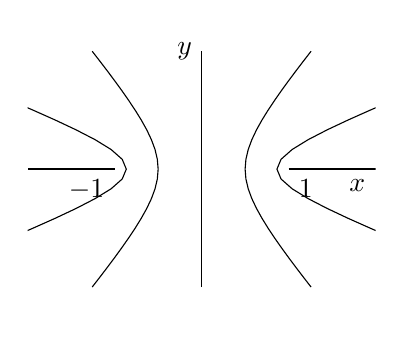
\begin{tikzpicture}
\begin{axis}[small,width=6cm,axis lines*=middle,axis line style={draw=none},ticks=none,xmin=-2,xmax=2]
\addplot[domain=-2:2] ({cos(30)*sqrt(1+x^2/sin(30)^2)},{x});
\addplot[domain=-2:2] ({-cos(30)*sqrt(1+x^2/sin(30)^2)},{x});
\addplot[domain=-2:2] ({cos(60)*sqrt(1+x^2/sin(60)^2)},{x});
\addplot[domain=-2:2] ({-cos(60)*sqrt(1+x^2/sin(60)^2)},{x});
\draw[thick] (axis cs:1,0)node[below right]{$1$}--(axis cs:2,0)node[below left]{$x$};
\draw[thick] (axis cs:-1,0)node[below left]{$-1$}--(axis cs:-2,0);
\draw(axis cs:0,-2)--(axis cs:0,2)node[left]{$y$};
\end{axis}
\end{tikzpicture}
\caption*{(الف)}
\end{subfigure}%
\begin{subfigure}{0.5\textwidth}
\centering
\begin{tikzpicture}
\begin{axis}[small,width=6cm,axis lines*=middle,axis line style={draw=none},ticks=none,xmin=-2,xmax=2]
\addplot[domain=-2:2] ({cos(30)*sqrt(1+x^2/sin(30)^2)},{x});
\addplot[domain=-2:2] ({cos(60)*sqrt(1+x^2/sin(60)^2)},{x});
\draw[thick] (axis cs:1,0)node[below right]{$1$}--(axis cs:2,0)node[below left]{$x$};
\draw[thick] (axis cs:0,-2)--(axis cs:0,2)node[left]{$y$};
\draw(axis cs:0,0)node[left]{$0$}--(axis cs:0.2,0);
\end{axis}
\end{tikzpicture}
\caption*{(ب)}
\end{subfigure}
\begin{subfigure}{0.5\textwidth}
\centering
\begin{tikzpicture}
\begin{axis}[small,width=6cm,axis lines*=middle,axis line style={draw=none},ticks=none,xmin=-2,xmax=2]
\addplot[thick,domain=-2:2] ({cos(30)*sqrt(1+x^2/sin(30)^2)},{x});
\addplot[thick,domain=-2:2] ({-cos(30)*sqrt(1+x^2/sin(30)^2)},{x});
\addplot[domain=-2:2] ({cos(60)*sqrt(1+x^2/sin(60)^2)},{x});
\addplot[domain=-2:2] ({-cos(60)*sqrt(1+x^2/sin(60)^2)},{x});
\draw(axis cs:-1,0)node[ocirc]{}node[left]{$-1$};
\draw(axis cs:1,0)node[ocirc]{}node[right]{$1$};
\draw(axis cs:0,-2)--(axis cs:0,2)node[left]{$y$};
\draw(axis cs:0,0)node[ocirc]{};
\draw(axis cs:1.5,0)--(axis cs:2,0)node[below]{$x$};
\end{axis}
\end{tikzpicture}
\caption*{(پ)}
\end{subfigure}
\caption{شکل برائے سوال \حوالہ{سوال_مخفی_قوہ_تین_طرز_الف}}
\label{شکل_سوال_مخفی_قوہ_تین_طرز_الف}
\end{figure}
\انتہا{سوال}
%===========================
\ابتدا{سوال}\quad
دکھائیں کہ \عددی{F(z)=\cosh^{-1} z} کو دو ہم ماسکہ ترخیمی نلکیوں کا مخلوط مخفی قوہ تصور کیا جا سکتا ہے۔\\
جواب:\quad
\begin{align*}
z=x+iy=\cosh(u+iv)=\cosh u\cos v+i\sinh u\sin v,\,\, \frac{x^2}{\cosh^2 u}+\frac{y^2}{\sinh^2 u}=1
\end{align*} 
یوں ہم قوہ خطوط \عددی{u=\text{مستقل}} ہم ماسکہ ترخیم ہیں۔
\انتہا{سوال}
%============================
\ابتدا{سوال}\شناخت{سوال_مخفی_قوہ_دو_نلکی}\quad
شکل \حوالہ{شکل_سوال_مخفی_قوہ_دو_نلکی} میں لامتناہی لمبائی کے دو نلکیاں دکھائی گئی ہیں۔بایاں نلکی پر \عددی{u=-1} اور دایاں نلکی پر \عددی{u=1} ہے۔نلکیوں کے درمیان خطہ میں مخفی قوہ \عددی{u} تلاش کریں۔ اشارہ۔ سوال \حوالہ{سوال_مخفی_قوہ_دو_منبع_لکیریں} کا نتیجہ استعمال کریں۔
\begin{figure}
\centering
\begin{tikzpicture}
\draw(-3,0)--(3,0)node[right]{$x$};
\draw(0,-1.5)--(0,1.5)node[left]{$y$};
\draw[thick](-5/3,0) circle (1);
\draw[thick](5/3,0) circle (1);
\draw[-stealth](-5/3,0)node[ocirc]{}node[below,xshift={(-0.1cm)}]{$-\tfrac{5}{3}$}--++(120:1)node[pos=0.5,fill=white,font=\small]{$r=1$};
\draw[-stealth](5/3,0)node[ocirc]{}node[below]{$\tfrac{5}{3}$}--++(60:1)node[pos=0.5,fill=white,font=\small]{$r=1$};
\draw(0,0)node[ocirc]{};
\end{tikzpicture}
\caption{شکل برائے سوال \حوالہ{سوال_مخفی_قوہ_دو_نلکی}}
\label{شکل_سوال_مخفی_قوہ_دو_نلکی}
\end{figure}
\انتہا{سوال}
%===========================

\حصہ{دو بعدی بہاو سیال}
ہارمونی تفاعل بہاو سیال میں کلیدی کردار ادا کرتے ہیں۔آئیں غیر چپچپا سیال کا دو بعدی برقرار بہاو پر غور کرتے ہیں۔یہاں "دو بعدی" کا مطلب ہے کہ \عددی{xy} مستوی کے متوازی تمام سطحوں میں سیال کی حرکت یکساں ہے اور حرکت ان سطحوں کے متوازی ہے۔ایسی صورت میں صفر \عددی{xy} سطح میں حرکت پر غور کرنا کافی ہو گا۔"بر قرار" کا مطلب ہے کہ  سمتی رفتار وقت کا تابع نہیں ہے۔

کسی بھی نقطہ \عددی{(x,y)} پر بہاو کی سمتی رفتار پائی جائے گی جس کو اس کی مقدار اور سمت سے ظاہر کیا جا سکتا ہے لہٰذا سمتی رفتار  ایک سمتیہ ہو گا۔چونکہ مخلوط سطح میں کوئی بھی عدد \عددی{a} ایک سمتیہ کو ظاہر کرتا ہے (جو مبدا سے عدد \عددی{a} کی مطابقتی مقام تک کا سمتیہ ہو گا) لہٰذا ہم بہاو کی سمتی رفتار کو مخلوط متغیرہ سے ظاہر کر سکتے ہیں مثلاً
\begin{align}
V=V_1+iV_2
\end{align} 
جہاں مخلوط سطح پر سمتی رفتار کے \عددی{x} اور \عددی{y} سمت میں  اجزاء بالترتیب \عددی{V_1} اور \عددی{V_2} ہوں گے اور \عددی{V} حرکت کرتے ذرات کی راہ کو مماسی ہو گا۔ایسی راہ کو \اصطلاح{سمت بہاو}\فرہنگ{سمت بہاو}\حاشیہب{streamline}\فرہنگ{streamline} کہتے ہیں (شکل \حوالہ{شکل_مخفی_سمتی_رفتار_سیال}-الف)۔
\begin{figure}
\centering
\begin{subfigure}{0.5\textwidth}
\centering
\begin{tikzpicture}
\draw(0,0)--++(4,0)node[right]{$x$};
\draw(0,0)--++(0,2.5)node[left]{$y$};
\draw[->-=0.15](0.4,0.4) to [out=50,in=-180]coordinate[pos=0.4](kA)coordinate[pos=0.15](kC) (4,2);
\draw(kC)node[right]{\RL{سمت بہاو}};
\draw[-latex](kA)--++(28:1.5)coordinate(kB)node[above]{$V$};
\path[name path=kPa] (kB)--++(-2,0);
\path[name path=kPb] (kA)--++(0,1);
\draw[-latex,dashed,name intersections={of=kPa and kPb}](kA)--(intersection-1)node[left]{$V_2$};
\draw[dashed](kB)--(intersection-1);
\path[name path=kPa] (kB)--++(0,-1);
\path[name path=kPb] (kA)--++(2,0);
\draw[-latex,dashed,name intersections={of=kPa and kPb}](kA)node[ocirc,solid]{}--(intersection-1)node[below]{$V_1$};
\draw[dashed](kB)--(intersection-1);
\end{tikzpicture}
\caption*{(الف) سمتی رفتار}
\end{subfigure}%
\begin{subfigure}{0.5\textwidth}
\centering
\begin{tikzpicture}
\draw(0,0)--(4,0)node[right]{$x$};
\draw(0,0)--(0,2.5)node[left]{$y$};
\draw(0.4,0.4)node[above]{$C$} to [out=10,in=-110]coordinate[pos=0.4](kA) (2.5,2.5);
\draw[-latex](kA)--++(-10:2)node[right]{$V$}coordinate(kB);
\path(kA)--++(39:1.5)coordinate(kE);
\path(kB)--($(kA)!(kB)!(kE)$)coordinate(kF);
\draw[-latex,dashed] (kA)node[ocirc,solid]{}--(kF)node[right]{$V_m$};
\draw[dashed](kB)--(kF);
\draw([shift={(-10:0.5)}]kA) arc (-10:39:0.5);
\draw(kA)++(10:0.8)node[]{$\alpha$};
\end{tikzpicture}
\caption*{(ب) منحنی \عددی{C} کو سمتی رفتار کا مماسی جزو}
\end{subfigure}%
\caption{سمت بہاو اور سمتی رفتار}
\label{شکل_مخفی_سمتی_رفتار_سیال}
\end{figure}

اب کسی ایک ہموار منحنی \عددی{C} پر غور کریں جس کی  لمبائی قوس کو ہم \عددی{s} سے ظاہر کرتے ہیں۔فرض کریں کہ \عددی{C} کو مماسی  سمتی رفتار \عددی{V} کا  جزو حقیقی متغیرہ  \عددی{V_m} ہے (شکل \حوالہ{شکل_مخفی_سمتی_رفتار_سیال}-ب) تب \عددی{C} پر \عددی{s} کی بڑھتی رخ خطی تکمل
\begin{align}
\int_C V_m\dif s
\end{align}
کو \عددی{C} پر سیال کی \اصطلاح{دائری بہاو}\فرہنگ{بہاو!دائری}\فرہنگ{دائری بہاو}\حاشیہب{circulation}\فرہنگ{circulation} کہتے ہیں۔دائری بہاو کو \عددی{C} کی لمبائی سے تقسیم کرنے سے منحنی \عددی{C} پر اوسط سمتی رفتار\حاشیہد{اوسط قیمتوں کی تعریفیں درج ذیل ہیں۔\\
$\,=\tfrac{1}{b-a}\int_a^b f(x)\dif x\,$
 وقفہ \عددی{a\le x\le b} پر \عددی{f} کی اوسط قیمت ہے۔\\
$\,=\tfrac{1}{l}\int_C f(s)\dif s\,$
\عددی{C} پر \عددی{f} کی اوسط قیمت ہے جہاں \عددی{C} کی لمبائی \عددی{l} ہے۔\\
$\,=\tfrac{1}{A}\iint\limits_D f(x,y)\dif x\dif y\,$ 
\عددی{D} میں \عددی{f} کی اوسط قیمت ہے جہاں \عددی{D} کا رقبہ \عددی{A} ہے۔
} 
 حاصل ہوتی ہے۔اب شکل \حوالہ{شکل_مخفی_سمتی_رفتار_سیال} سے
\begin{align*}
V_m=\abs{V}\cos \alpha
\end{align*}
لکھا جا سکتا ہے۔نتیجتاً  \عددی{C} کے اکائی مماسی سمتیہ (حصہ \حوالہ{حصہ_نقش_محافظ_زاویہ_نقش})
\begin{align*}
\frac{\dif z}{\dif s}=\frac{\dif x}{\dif s}+i\frac{\dif y}{\dif s}
\end{align*}
اور \عددی{V} کا اندرونی ضرب (حصہ \حوالہ{حصہ_سمتیہ_اندرونی_ضرب_فضا}) \عددی{V_m} ہو گا جہاں \عددی{C} کو \عددی{z(s)=x(s)+iy(s)} سے ظاہر کیا جائے گا۔اس طرح \عددی{V_m\dif s} کو 
\begin{align*}
V_m\dif s=V\cdot \dif z=V_1\dif x+V_2\dif y\quad \quad (\dif z=\dif x+i\dif y)
\end{align*}
لکھا جا سکتا ہے۔(یہاں اچھی طرح سمجھ سمجھ لیں کہ یہ دو سمتیات کے مابین غیر سمتی ضرب ہے نا کہ مخلوط ضرب۔)

اب فرض کریں کہ \عددی{C} ایک بند منحنی ہے یعنی سادہ تعلق دائرہ کار \عددی{D} کا سرحد۔ تب اگر ایسا دائرہ کار جس میں \عددی{D} اور \عددی{C} شامل ہوں  میں \عددی{V} کے استمراری جزوی تفرق پائے جاتے ہوں  تب مسئلہ گرین (حصہ \حوالہ{حصہ_خطی_تکمل_دوہرا_خطی_تبادل}) کے تحت \عددی{C} پر دائری بہاو کو دوہرا تکمل
\begin{align}
\int\limits_C (V_1\dif x+V_2\dif y)=\iint\limits_D \big(\frac{\partial V_2}{\partial x}-\frac{\partial V_1}{\partial y}\big)\dif x\dif y
\end{align}
کی صورت میں لکھا جا سکتا ہے۔دائیں ہاتھ تکمل کے اندر تفاعل کا ایک سادہ طبعی مطلب ہے جس پر اب غور کرتے ہیں۔فرض کریں کہ \عددی{C} ایک دائرہ ہے جس کا  رداس \عددی{r}  ہے۔تب دائری بہاو کو \عددی{2\pi r} سے تقسیم کرنے سے  سیال کی \عددی{C} پر اوسط سمتی رفتار حاصل ہو گی جس کو \عددی{r} سے تقسیم کرتے ہوئے  دائرے کی محور پر سیال کی زاویائی سمتی رفتار \عددی{\omega_0} حاصل ہوتی ہے۔
\begin{align}\label{مساوات_مخفی_قوہ_گرداب_الف}
\omega_0=\frac{1}{\pi r^2}\iint\limits_D \frac{1}{2}\big(\frac{\dif V_2}{\dif x}-\frac{\dif V_1}{\dif y}\big)\dif x\dif y
\end{align}
دایاں ہاتھ قرص \عددی{D} جس کی سرحد \عددی{C} ہے  پر درج ذیل تفاعل کی اوسط قیمت\حاشیہد{اوسط کی تعریف کے لئے گزشتہ حاشیہ دیکھیں} ہے۔
\begin{align}
\omega=\frac{1}{2}\big(\frac{\dif V_2}{\dif x}-\frac{\dif V_1}{\dif y}\big)
\end{align} 
تفاعل \عددی{\omega} \اصطلاح{گھومنا}\فرہنگ{گھومنا}\حاشیہب{rotation}\فرہنگ{rotation} کہلاتا ہے جبکہ \عددی{2\omega} کو حرکت کی \اصطلاح{گردابیت}\فرہنگ{گردابیت}\حاشیہب{vorticity}\فرہنگ{vorticity} کہتے ہیں۔اگر \عددی{r\to 0} ہو تب مساوات \حوالہ{مساوات_مخفی_قوہ_گرداب_الف} کے دایاں ہاتھ کی حد، \عددی{C} کی مرکز پر  \عددی{\omega} کی قیمت دے گی۔یوں اگر دائرہ \عددی{C} سکڑ کر نقطہ \عددی{(x,y)} مانند رہ جائے تب سیال کے دائری ٹکڑے کی زاویائی سمتی رفتار کی تحدیدی قیمت  \عددی{w(x,y)} ہو گی۔ہم کہہ سکتے ہیں کہ اگر سیال کا کروی ٹکرا یک دم ٹھوس صورت اختیار کرے اور ساتھ ہی باقی تمام سیال ہٹا دیا جائے تب اس ٹکڑے کی زاویائی سمتی رفتار \عددی{\omega}  ہو گی (حصہ \حوالہ{حصہ_سمتی_تفرق_گردش} دیکھیں)۔

ہم صرف \اصطلاح{نا گھومتے}\فرہنگ{نا گھومتا}\حاشیہب{irrotational}\فرہنگ{irrotational} سیال پر غور کرتے ہیں یعنی ایسا سیال جس کا \عددی{\omega} پورے خطہ \عددی{D}  پر صفر کے برابر ہو،
\begin{align*}
\frac{\dif V_2}{\dif x}-\frac{\dif V_1}{\dif y}=0
\end{align*} 
جہاں تفرق کی موجودگی اور استمرار فرض کی گئی ہے۔

ہم مزید فرض کرتے ہیں کہ سیال داب نا پذیر ہے۔تب ہر اس خطہ میں،جس میں نا کوئی \اصطلاح{منبع}\فرہنگ{منبع}\حاشیہب{source}\فرہنگ{source} (سوال \حوالہ{سوال_مخلوط_مخفی_قوہ_منبع_گڑھا_الف}) اور نا ہی کوئی \اصطلاح{گڑھا}\فرہنگ{گڑھا}\حاشیہب{sink}\فرہنگ{sink} پایا جاتا ہو یعنی جس میں سیال نا پیدا ہوتا ہو اور نا ہی غائب ہوتا ہو، مساوات \حوالہ{مساوات_سمتی_تفرق_پھیلاو_صفر} کے تحت
\begin{align}\label{مساوات_مخفی_قوہ_داب_نا_پذیر_الف}
\frac{\dif V_1}{\dif x}+\frac{\dif V_2}{\dif y}=0
\end{align}
ہو گا۔

اگر \عددی{D} سادہ تعلق خطہ ہو اور بہاو نا گھومنے والی ہو تب مسئلہ \حوالہ{مسئلہ_خطی_تکمل_اصول_قطعیت} کے تحت خطی تکمل
\begin{align}
\int_C\, (V_1\dif x+V_2\dif y)
\end{align}
\عددی{D} میں راہ کا تابع نہیں ہو گا۔یوں \عددی{D} میں مقررہ نقطہ \عددی{(a,b)} سے \عددی{D} میں متغیر نقطہ \عددی{(x,y)} تک تکمل حاصل کرنے سے  نقطہ \عددی{(x,y)} کا تابع تفاعل مثلاً \عددی{\Phi(x,y)} حاصل ہو گا:
\begin{align}
\Phi(x,y)=\int\limits_{(a,b)}^{(x,y)} (V_1\dif x+V_2\dif y)
\end{align}
تفاعل \عددی{\Phi(x,y)} کو حرکت کی \اصطلاح{سمتی رفتار مخفی قوہ}\فرہنگ{سمتی رفتار!مخفی قوہ}\فرہنگ{مخفی قوہ!سمتی رفتار}\حاشیہب{velocity potential}\فرہنگ{velocity!potential} کہتے ہیں۔اب چونکہ درج بالا تکمل راہ کا تابع نہیں  ہے لہٰذا \عددی{V_1\dif x+V_2\dif y} قطعی تفرق (حصہ \حوالہ{حصہ_خطی_تکمل_راہ_سے_آزاد_تکمل}) ہو گا یعنی یہ تفاعل \عددی{\Phi(x,y)} کا تفرق ہو گا:
\begin{align}
V_1\dif x+V_2\dif y=\frac{\partial \Phi}{\partial x}\dif x+\frac{\partial \Phi}{\partial y}\dif y
\end{align}
یوں 
\begin{align}\label{مساوات_مخفی_قوہ_ڈھلوان_مخفی_الف}
V_1=\frac{\partial \Phi}{\partial x},\quad V_2=\frac{\partial \Phi}{\partial y}
\end{align}
ہو گا لہٰذا سمتی رفتار سمتیہ تفاعل \عددی{\Phi(x,y)} کی ڈھلوان (حصہ \حوالہ{حصہ_الاحصاء_ڈھلوان}) ہو گا۔
\begin{align}
V=V_1+iV_2=\frac{\partial \Phi}{\partial x}+i\frac{\partial \Phi}{\partial y}
\end{align}
منحنی \عددی{\Phi(x,y)=\text{مستقل}} کو \اصطلاح{ہم قوہ خط}\فرہنگ{ہم قوہ!خط}\حاشیہب{equipotential lines}\فرہنگ{equipotential!lines} کہتے ہیں۔چونکہ \عددی{\Phi} کی ڈھلوان \عددی{V} ہے لہٰذا (\عددی{V\ne 0} کی صورت میں) ہر نقطہ پر \عددی{V} اور اس نقطہ سے گزرتا ہم قوہ خط آپس میں قائمہ الزاویہ ہوں گے۔ 

مساوات \حوالہ{مساوات_مخفی_قوہ_ڈھلوان_مخفی_الف} کو مساوات \حوالہ{مساوات_مخفی_قوہ_داب_نا_پذیر_الف} میں پر کرنے سے ہم دیکھتے ہیں کہ \عددی{\Phi} مساوات لاپلاس
\begin{align*}
\nabla^{\,2}\Phi=\frac{\partial^{\,2}\Phi}{\partial x^2}+\frac{\partial^{\,2}\Phi}{\partial y^2}=0
\end{align*}
کو مطمئن کرتا ہے۔فرض کریں کہ \عددی{\Phi(x,y)} کا جوڑی دار ہارمونی تفاعل \عددی{\Psi(x,y)} ہو، تب[(ماسوائے اس نقطہ پر جہاں (مساوات \حوالہ{مساوات_مخفی_قوہ_مخلوط_تفاعل_مخفی_بہاو} میں دیا گیا) \عددی{F'(z)=0} ہو] ہر ایک نقطہ پر منحنیات
\begin{align*}
\Psi(x,y)=\text{مستقل}
\end{align*}
اور ہم قوہ خطوط \عددی{\Phi(x,y)=\text{مستقل}} آپس میں قائمہ الزاویہ ہوں گی۔یوں  منحنیات \عددی{\Psi(x,y)=\text{مستقل}} کے مماس کی سمت اور سیال کی سمتی رفتار کی سمت ایک جیسی ہوں گی۔نتیجتاً منحنیات \عددی{\Psi(x,y)=\text{مستقل}} سیال کی سمت بہاو خط ہوں گے۔تفاعل \عددی{\Psi(x,y)=\text{مستقل}} کو بہاو کا \اصطلاح{تفاعل بہاو}\فرہنگ{تفاعل!بہاو}\حاشیہب{stream function}\فرہنگ{stream!function} کہتے ہیں۔

ہم فرض کرتے ہیں کہ \عددی{\Phi} اور \عددی{\Psi} دونوں کے استمراری دوہرا جزوی تفرق پائے جاتے ہیں۔تب مخلوط تفاعل 
\begin{align}\label{مساوات_مخفی_قوہ_مخلوط_تفاعل_مخفی_بہاو}
F(z)=\Phi(x,y)+i\Psi(x,y)
\end{align}
بہاو کے خطہ میں تحلیلی ہو گا۔اس تفاعل کو بہاو کی \اصطلاح{مخلوط مخفی قوہ}\فرہنگ{مخلوط مخفی قوہ}\حاشیہب{complex potential}\فرہنگ{potential!complex} کہتے ہیں۔\عددی{\Phi} اور \عددی{\Psi} کے ساتھ علیحدہ علیحدہ کام کرنے سے مخلوط مخفی قوہ کے ساتھ کام کرنا زیادہ آسان ثابت ہوتا ہے۔

مساوات \حوالہ{مساوات_مخفی_قوہ_مخلوط_تفاعل_مخفی_بہاو} کا تفرق لے کر اور مساوات کوشی ریمان استعمال کرتے ہوئے بہاو کی سمتی رفتار حاصل کی جا سکتی ہے۔ یوں
\begin{align*}
F'(z)=\frac{\partial \Phi}{\partial x}+i\frac{\partial \Psi}{\partial x}=\frac{\partial \Phi}{\partial x}-i\frac{\partial \Phi}{\partial y}=V_1-iV_2
\end{align*}
حاصل ہوتا ہے جس سے
\begin{align}\label{مساوات_مخفی_قوہ_سیال_اہم_مساوات}
V=V_1+iV_2=\overline{F'(z)}
\end{align}
لکھا جا سکتا ہے۔

اس طرح دو بعدی، نا گھومنے والی، داب نا پذیر سیال کی برقرار بہاو کو تحلیلی تفاعل کی صورت میں بیان کیا جا سکتا ہے اور مخلوط تجزیہ کے تراکیب، مثلاً محافظ زاویہ نقش، استعمال کیے جا سکتے ہیں۔  

چونکہ وہ سرحد جس کو بہاو پار نہ کر سکتا ہو بہاو سمت ہو گا لہٰذا سرحدی شرائط مسائل میں بہاو سمت تفاعل \عددی{\Psi} نہایت اہم  ثابت ہوتا ہے۔زیر محافظ زاویہ نقش، بہاو سمت کا تبادل سطح عکس میں بہاو سمت پر ہو گا۔پیچیدہ بہاو کے حصول اور ان پر غور کے لئے سادہ بہاو کا میل زیر استعمال لایا جا سکتا ہے۔دو بہاو \عددی{F_1}، \عددی{F_2} کا مجموعہ \عددی{F=F_1+F_2} دونوں بہاو کی سمتی رفتار کی سمتیات کا سمتی مجموعہ سے حاصل بہاو کا مخلوط مخفی قوہ ہو گا۔چونکہ مساوات لاپلاس خطی اور متجانس ہے  لہٰذا دو ہارمونی تفاعل کا مجموعہ بھی  ہارمونی ہو گا۔

دھیان رہے کہ اگرچہ برقی سکون میں دی گئی سرحدیں (موصل سطحیں) ہم قوہ خطوط ہوں گی، ماقوا حرکیات میں یہ سرحدیں بہاو سمت ہوں گی اور ہم قوہ خطوط کے قائمہ الزاویہ ہوں گی۔    

آئیں ایک عمومی مثال کو دیکھیں۔مزید مسائل سوالات میں پیش کیے گئے ہیں۔

%============================
\ابتدا{مثال}\شناخت{مثال_مخفی_قوہ_کونے_پر_بہاو}\quad \موٹا{کونے کے ساتھ بہاو}\\
مخلوط مخفی قوہ 
\begin{align}
F(z)=z^2=x^2-y^2+i2xy
\end{align}
ایسی بہاو کو ظاہر کرتا ہے  جس کے ہم قوہ خطوط درج ذیل  قطع زائد
\begin{align*}
\Phi=x^2-y^2=\text{مستقل}
\end{align*}
اور بہاو سمت درج ذیل  قطع زائد
\begin{align*}
\Psi=2xy=\text{مستقل}
\end{align*}
ہوں گی۔مساوات \حوالہ{مساوات_مخفی_قوہ_سیال_اہم_مساوات} سے درج ذیل سمتی رفتار سمتیہ حاصل ہوتا ہے۔
\begin{align*}
V=2\bar{z}=2(x-iy),\quad \implies\quad V_1=2x,\quad V_2=-2y
\end{align*}
رفتار (سمتیہ کی مقدار) درج ذیل ہو گی۔
\begin{align*}
\abs{V}=\sqrt{V_1^2+V_2^2}=2\sqrt{x^2+y^2}
\end{align*}
اس بہاو کو ایسی ندی کی بہاو تصور کیا جا سکتا ہے جس کے اطراف کارتیسی محدد کے مثبت محور اور قطع زائد مثلاً \عددی{xy=1} ہو (شکل \حوالہ{شکل_مخفی_قوہ_کونے_پر_بہاو})۔ہم دیکھتے ہیں کہ کسی بہاو سمت \عددی{S} پر  نقطہ \عددی{N} پر رفتار کم تر ہو گا۔یہ وہ نقطہ ہے جہاں ندی کی عمودی تراش رقبہ زیادہ سے زیادہ ہو گا۔
\begin{figure}
\centering
\begin{tikzpicture}
\draw[very thick](0,2)--(0,0)node[below]{$0$}--(3,0);
\draw(3.2,0)--(4,0)node[right]{$x$};
\draw(0,2.2)--(0,2.75)node[left]{$y$};
\draw[very thick,domain=0.5:3] plot ({\x},{1/\x});
\draw[->-=0.25,smooth,domain=1/3:3] plot ({\x},{2/(3*\x)});
\draw[->-=0.25,smooth,name path=kC,domain=1/6:3] plot ({\x},{1/(3*\x)});
\draw[name path=kB,dashed](0,0)--(45:1.4);
\draw[name intersections={of=kC and kB}] (intersection-1)node[ocirc]{}node[yshift={(-0.3cm)}]{$N$};
\draw(1/6,2)node[above]{$S$};
\end{tikzpicture}
\caption{کونے پر بہاو}
\label{شکل_مخفی_قوہ_کونے_پر_بہاو}
\end{figure}
\انتہا{مثال}
%============================

\حصہء{سوالات}

%==============
\ابتدا{سوال}\شناخت{سوال_مخفی_قوہ_کونے_پر_بہاو}\quad \موٹا{(متوازی بہاو)} \quad
دکھائیں کہ \عددی{F(z)=Kz} (جہاں \عددی{K} مثبت حقیقی ہے) دائیں رخ یکساں بہاو کو ظاہر کرتی ہے جس کو دو متوازی لکیروں (تین بعدی فضا میں دو متوازی چادروں) کے درمیان یکساں بہاو تصور کیا جا سکتا ہے (شکل \حوالہ{شکل_مخفی_قوہ_یکساں_متوازی_بہاو})۔ سمتی رفتار سمتیہ، بہاو سمت اور ہم قوہ خطوط تلاش کریں۔
\begin{figure}
\centering
\begin{tikzpicture}
\draw (2.5,0)--(3,0)node[right]{$x$};
\draw(0,-1.2)--(0,1.5)node[left]{$y$};
\draw[thick](-1,-1)--(2,-1);
\draw[thick](-1,1)--(2,1);
\draw[->-=0.75](-1,-0.5)--(2,-0.5);
\draw[->-=0.75](-1,0)--(2,0);
\draw[->-=0.75](-1,0.5)--(2,0.5);
\end{tikzpicture}
\caption{یکساں متوازی بہاو}
\label{شکل_مخفی_قوہ_یکساں_متوازی_بہاو}
\end{figure}

جواب:\quad
$V=V_1=K,\,\, Ky=\text{مستقل},\,\, Kx=\text{مستقل}$
\انتہا{سوال}
%============================
\ابتدا{سوال}\quad 
دکھائیں کہ کونے پر بہاو کو \عددی{F(z)=iz^2} ظاہر کرتی ہے۔بہاو سمت اور ہم قوہ خطوط تلاش کریں اور انہیں ترسیم کریں۔ سمتی رفتار سمتیہ \عددی{V} تلاش کریں۔
\انتہا{سوال}
%=======================
\ابتدا{سوال}\quad
مثال \حوالہ{مثال_مخفی_قوہ_کونے_پر_بہاو} کی بہاو محافظ نقش کی استعمال سے سوال \حوالہ{سوال_مخفی_قوہ_کونے_پر_بہاو} سے حاصل کریں۔آپ کو ربع اول کا نقش بالائی نصف مستوی پر کرنا ہو گا۔
\انتہا{سوال}
%=======================
\ابتدا{سوال}\quad
مخلوط مخفی قوہ \عددی{F(z)=z^3} کے بہاو سمت اور ہم قوہ خطوط تلاش کریں۔انہیں ترسیم کریں۔سمتی رفتار سمتیہ \عددی{V} تلاش کریں اور وہ تمام نقطے دریافت کریں جہاں یہ سمتیہ \عددی{x} محور کے متوازی ہے۔
\انتہا{سوال}
%======================
سوال \حوالہ{سوال_مخفی_قوہ_مخلوط_الف} تا سوال \حوالہ{سوال_مخفی_قوہ_مخلوط_ب} میں دی گئی مخلوط مخفی قوہ \عددی{F(z)} پر غور کریں۔ہم قوہ خطوط اور بہاو سمت کی ترسیم کھینچیں۔سمتی رفتار سمتیہ \عددی{V} تلاش کریں اور وہ تمام نقطے دریافت کریں جہاں یہ سمتیہ \عددی{x} محور کے متوازی ہے۔

%========================
\ابتدا{سوال}\شناخت{سوال_مخفی_قوہ_مخلوط_الف}\quad
$F=iz$\\
جواب:\quad
منفی \عددی{y} محور کے رخ متوازی بہاو۔ \عددی{V=-i}
\انتہا{سوال}
%=========================
\ابتدا{سوال}\quad
$\,F=-ikz\,$
\عددی{k} حقیقی عدد صحیح ہے۔
\انتہا{سوال}
%========================
\ابتدا{سوال}\quad
$F=(1+i)z$\\
جواب:\quad
\عددی{y=-x} کی رخ متوازی بہاو۔ \عددی{V=1-i}
\انتہا{سوال}
%===========================
\ابتدا{سوال}\quad
$F=z^2+z$
\انتہا{سوال}
%===========================
\ابتدا{سوال}\شناخت{سوال_مخفی_قوہ_مخلوط_ب}\quad
$F=iz^3$\\
جواب:\quad
\عددی{V=-6xy+3i(y^2-x^2)}؛ \عددی{y=x} اور \عددی{y=-x} پر \عددی{V_2=0} ہے۔
\انتہا{سوال}
%===========================
\ابتدا{سوال}\شناخت{سوال_مخلوط_مخفی_قوہ_منبع_گڑھا_الف}\quad \موٹا{(منبع اور گڑھا)} \quad 
مخلوط مخفی قوہ \عددی{F(z)=\tfrac{c}{2\pi}\ln z} پر غور کریں جہاں \عددی{c} حقیقی مثبت ہے۔دکھائیں کہ \عددی{V=\tfrac{c}{2\pi r^2}(x+iy)} ہو گا جہاں \عددی{r=\sqrt{x^2+y^2}} ہے۔ یہ رداسی باہر رخ بہاو کو ظاہر کرتی ہے (شکل \حوالہ{مساوات_مخلوط_مخفی_قوہ_نقطہ_منبع}-الف)۔یہ نقطہ \عددی{z=0} پر \اصطلاح{منبع}\فرہنگ{منبع}\حاشیہب{source}\فرہنگ{source} کا مخفی قوہ ہو گا (یعنی فضا میں \عددی{x=0}، \عددی{y=0} پر منبع لکیر)۔مستقل \عددی{c} کو منبع کا \اصطلاح{زور} یا \اصطلاح{اخراج} کہا جاتا ہے۔ اگر \عددی{c} منفی ہو تب ہم کہتے ہیں کہ \عددی{z=0} پر بہاو کا \اصطلاح{گڑھا}\فرہنگ{گڑھا}\حاشیہب{sink}\فرہنگ{sink} پایا جاتا ہے۔اب بہاو رداسی اندر رخ  کو ہے اور مخلوط مخفی قوہ کے نقطہ نادر \عددی{z=0} پر بہاو غائب ہو جاتی ہے۔\\
جواب:\quad
$\tfrac{\dif F}{\dif z}=\tfrac{c}{2\pi z}=\tfrac{c}{2\pi(x+iy)}=\tfrac{c(x-iy)}{2\pi(x^2+y^2)},\quad V=\overline{\tfrac{\dif F}{\dif z}}=\tfrac{c(x+iy)}{2\pi(x^2+y^2)}$
%
\begin{figure}
\centering
\begin{subfigure}{0.5\textwidth}
\centering
\begin{tikzpicture}
\pgfmathsetmacro{\ang}{30}
\pgfmathsetmacro{\len}{1.5}
\foreach \m in {0,1,2,3,4,5,6,7,8,9,10,11}{
\draw[->-=0.6](0,0)--(\m*\ang:\len);}
\draw[dashed] (0,0) circle (0.5);
\draw[dashed] (0,0)node[ocirc]{} circle (1);
\draw(1.75,0)--(2,0)node[below]{$x$};
\draw(0,1.6)--(0,1.75)node[left]{$y$};
\end{tikzpicture}
\caption*{(الف) نقطہ منبع}
\end{subfigure}%
\begin{subfigure}{0.5\textwidth}
\centering
\begin{tikzpicture}
\pgfmathsetmacro{\ang}{30}
\pgfmathsetmacro{\len}{1.5}
\foreach \m in {0,1,2,3,4,5,6,7,8,9,10,11}{
\draw[dashed](0,0)--++(\m*\ang:\len);}
\draw[->-=0.15](0,0) circle (0.25);
\draw[->-=0.15](0,0) circle (0.5);
\draw[->-=0.15](0,0) circle (0.75);
\draw[->-=0.15](0,0) circle (1);
\draw(0,0)node[ocirc]{};
\draw(1.5,0)--(2,0)node[below]{$x$};
\draw(0,1.5)--(0,1.75)node[left]{$y$};
\end{tikzpicture}
\caption*{(ب) بہاو گرداب}
\end{subfigure}
\caption{اشکال برائے سوال \حوالہ{سوال_مخلوط_مخفی_قوہ_منبع_گڑھا_الف} اور سوال \حوالہ{سوال_مخلوط_مخفی_قوہ_منبع_گڑھا_ب}}
\label{مساوات_مخلوط_مخفی_قوہ_نقطہ_منبع}
\end{figure}
\انتہا{سوال}
%========================
\ابتدا{سوال}\شناخت{سوال_مخلوط_مخفی_قوہ_منبع_گڑھا_ب}\quad \موٹا{(لکیر گرداب)}\quad
دکھائیں کہ \عددی{F(z)=-\tfrac{iK}{2\pi}\ln z} جہاں \عددی{K} حقیقی ہے، مبدا کے گرد گھڑی کی الٹ رخ بہاو کو ظاہر کرتی ہے (شکل \حوالہ{مساوات_مخلوط_مخفی_قوہ_نقطہ_منبع}-ب)۔  نقطہ \عددی{z=0} \اصطلاح{گرداب}\فرہنگ{گرداب}\حاشیہب{vortex}\فرہنگ{vortex} ہے۔ گرداب کے گرد ہر ایک چکر لگانے سے مخفی قوہ بڑھ جاتی ہے جہاں ہر مرتبہ  بڑھنے کی مقدار \عددی{K} ہو گی۔\\
جواب:\quad
$F=-\tfrac{iK}{2\pi}\ln (re^{i\theta})=-\tfrac{iK}{2\pi}(i\theta+\ln r)=\tfrac{K}{2\pi}(\theta-i\ln r)=\Phi+i\Psi$
\انتہا{سوال}
%=======================
\ابتدا{سوال}\شناخت{سوال_مخفی_قوہ_مخلوط_تلاش_الف}\quad
نقطہ \عددی{z=-a} پر اکائی زور کی منبع کے بہاو کا مخلوط مخفی قوہ تلاش کریں۔
\انتہا{سوال}
%======================
\ابتدا{سوال}\شناخت{سوال_مخفی_قوہ_مخلوط_تلاش_ب}\quad
دکھائیں کہ دو بہاو کے سمتی رفتار سمتیات کا سمتی مجموعہ حاصل کرنے سے  ایسا بہاو حاصل ہو گا جس کا مخلوط مخفی قوہ ان بہاو کے مخلوط مخفی قوہ کو جمع کرنے سے حاصل ہوتا ہے۔ 
\انتہا{سوال}
%====================
\ابتدا{سوال}\شناخت{سوال_مخفی_قوہ_مخلوط_تلاش_پ}\quad
سوال \حوالہ{سوال_مخفی_قوہ_مخلوط_تلاش_الف} اور سوال \حوالہ{سوال_مخفی_قوہ_مخلوط_تلاش_ب} کے مخفی قوہ جمع کرتے ہوئے بہاو سمت کی ترسیم کھینچیں۔
\انتہا{سوال}
%=====================
\ابتدا{سوال}\quad
\عددی{F(z)=\tfrac{1}{z}} کے بہاو کی بہاو سمت تلاش کریں۔دکھائیں کہ چھوٹے \عددی{\abs{a}} کے لئے  سوال \حوالہ{سوال_مخفی_قوہ_مخلوط_تلاش_پ} کے بہاو سمت موجودہ بہاو سمت کی طرح ہیں۔
\انتہا{سوال}
%==========================
\ابتدا{سوال}\شناخت{سوال_مخفی_قوہ_بہاو_الف}\quad
دکھائیں کہ \عددی{F(z)=\cosh^{-1} z} کے بہاو سمت،  ہم ماسکہ قطع زائد  ہوں گی جن کے ماسکہ \عددی{z=\mp 1} ہیں اور بہاو کو شگاف سے گزرتی بہاو تصور کیا جا سکتا ہے (شکل \حوالہ{شکل_مخفی_قوہ_شگاف_بہاو}-الف)۔
\begin{figure}
\centering
\begin{subfigure}{0.5\textwidth}
\centering
\begin{tikzpicture}
\begin{axis}[small,width=6cm,axis lines*=middle,axis line style={draw=none},ticks=none,xmin=-2,xmax=2]
\addplot[->-=0.6,domain=-2:2] ({cos(30)*sqrt(1+x^2/sin(30)^2)},{x});
\addplot[->-=0.6,domain=-2:2] ({-cos(30)*sqrt(1+x^2/sin(30)^2)},{x});
\addplot[->-=0.75,domain=-2:2] ({cos(60)*sqrt(1+x^2/sin(60)^2)},{x});
\addplot[->-=0.75,domain=-2:2] ({-cos(60)*sqrt(1+x^2/sin(60)^2)},{x});
\draw[thick] (axis cs:1,0)node[below right]{$1$}--(axis cs:2,0);
\draw[thick] (axis cs:-1,0)node[below left]{$-1$}--(axis cs:-2,0);
\draw[->-=0.8](axis cs:0,-2)--(axis cs:0,2);
\end{axis}
\end{tikzpicture}
\caption{شگاف سے بہاو}
\end{subfigure}%
\begin{subfigure}{0.5\textwidth}
\centering
\begin{tikzpicture}
\draw[->-=0.25] (0,0) circle (1.1276 and 0.521);
\draw[->-=0.25] (0,0) circle (1.543 and 1.175);
\draw[->-=0.25] (0,0) circle (1.888 and 1.6);
\draw[thick](-1,0)node[below]{$-1$}--(1,0)node[below]{$1$};
\end{tikzpicture}
\caption*{(ب) چادر کے گرد بہاو}
\end{subfigure}
\caption{اشکال برائے سوال \حوالہ{سوال_مخفی_قوہ_بہاو_الف} اور سوال \حوالہ{سوال_مخفی_قوہ_بہاو_ب}}
\label{شکل_مخفی_قوہ_شگاف_بہاو}
\end{figure}
\انتہا{سوال}
%=======================
\ابتدا{سوال}\شناخت{سوال_مخفی_قوہ_بہاو_ب}\quad
دکھائیں کہ \عددی{F(z)=\cos^{-1} z} کو ترخیم یا چادر (\عددی{z=-1} تا \عددی{z=1} سیدھی قطع) کے گرد بہاو کا مخلوط مخفی قوہ تصور کیا جا سکتا ہے۔دکھائیں کہ بہاو سمت ہم ماسکہ ترخیم ہیں جن کے ماسکہ \عددی{z=\mp 1} پر ہیں (شکل \حوالہ{شکل_مخفی_قوہ_شگاف_بہاو}-ب)۔
\انتہا{سوال}
%==========================
\ابتدا{سوال}\شناخت{سوال_مخفی_قوہ_بیلن_کے_گرد}\quad \موٹا{(بیلن کے گرد بہاو)}\quad
\عددی{F(z)=z+z^{-1}} پر غور کریں۔ \عددی{z=re^{i\theta}} لیتے ہوئے دکھائیں کہ سمتی قوہ \عددی{(r-r^{-1})\sin\theta=\text{مستقل}} ہیں اور سمتی قوہ \عددی{(r-r^{-1})\sin\theta=0} اکائی دائرہ اور \عددی{x} محور پر مشتمل ہے، اور بڑے \عددی{\abs{z}} کے لئے بہاو تقریباً یکساں اور متوازی ہے جس کو اکائی رداس کے بیلن کے گرد بہاو تصور کیا جا سکتا ہے (شکل \حوالہ{شکل_سوال_مخفی_قوہ_بیلن_کے_گرد} میں \عددی{K=0} صورت)۔ بہاو کا نقطہ ٹھراو تلاش کریں (جہاں سمتی رفتار صفر ہو گی)۔

جواب:\quad
نقطہ \عددی{z=-1} اور \عددی{z=1} پر \عددی{V=1-\bar{z}^{-1}=0} ہو گا۔
\انتہا{سوال}
%=======================
\ابتدا{سوال}\شناخت{سوال_مخفی_قوہ_بیلن_کے_گرد_ب}\quad \موٹا{(دائری بہاو کے ساتھ بیلن کے گرد بہاو)}\quad
سوال \حوالہ{سوال_مخلوط_مخفی_قوہ_منبع_گڑھا_ب} اور سوال \حوالہ{سوال_مخفی_قوہ_بیلن_کے_گرد} کے مخفی قوہ جمع کرتے ہوئے دکھائیں کہ بیلن کی سطح \عددی{\abs{z}=1} سمت بہاو ہے۔سمتی رفتار تلاش کریں اور دکھائیں کہ نقطہ ٹھراو
\begin{align*}
z=\frac{iK}{4\pi}\mp \sqrt{-\frac{K^2}{16\pi^2}+1}
\end{align*}
ہیں جو \عددی{K=0} کی صورت میں \عددی{z=\mp 1} دیتی ہے۔\عددی{K} بڑھانے سے دونوں نقطہ ٹھراو اکائی دائرہ پر اوپر رخ منتقل ہوں گے  حتیٰ کہ \عددی{K=4\pi} پر دونوں \عددی{z=i} پر آن ملیں گے۔اگر \عددی{K>4\pi}  کیا جائے تب ایک نقطہ ٹھراو خیالی محور پر بیلن کے باہر اور دوسرا خیالی محور پر بیلن کے اندر منتقل ہوتا ہے۔بیلن کے اندر نقطہ ٹھراو کی کوئی طبعی معنی نہیں ہے۔(شکل \حوالہ{شکل_سوال_مخفی_قوہ_بیلن_کے_گرد} میں \عددی{K=0} کے لئے نقطہ ٹھراو کو چھوٹے دائروں سے ظاہر کیا گیا ہے۔)\\
جواب:\quad
سمت بہاو 
$\Psi_1+\Psi_2=\sin\theta(r-r^{-1})+\tfrac{K}{2\pi}\ln r=c$
ہے جس کو شکل \حوالہ{شکل_سوال_مخفی_قوہ_بیلن_کے_گرد} میں مختلف \عددی{c} اور \عددی{K} کے لئے دکھایا گیا ہے۔
\انتہا{سوال}
%================
\begin{figure}
\centering
\begin{subfigure}{0.5\textwidth}
\centering
\begin{tikzpicture}[scale=0.75]
\begin{polaraxis}[ymax=4,axis lines=none]
\addplot[thick,domain=0:360,smooth]{1};
\pgfmathsetmacro{\ca}{0.25}
\addplot[domain=10:170,-<-=0.25] {(\ca+sqrt(\ca^2+4*(sin(x))^2)/(2*sin(x)))};
\addplot[domain=5:10] {(\ca+sqrt(\ca^2+4*sin(x)^2)/(2*sin(x)))};
\addplot[domain=1:5] {(\ca+sqrt(\ca^2+4*sin(x)^2)/(2*sin(x)))};
\addplot[domain=170:175] {(\ca+sqrt(\ca^2+4*sin(x)^2)/(2*sin(x)))};
\addplot[domain=175:179] {(\ca+sqrt(\ca^2+4*sin(x)^2)/(2*sin(x)))};
%
\addplot[domain=-10:-170,-<-=0.25] {(\ca+sqrt(\ca^2+4*(sin(-x))^2)/(2*sin(-x)))};
\addplot[domain=-5:-10] {(\ca+sqrt(\ca^2+4*sin(-x)^2)/(2*sin(-x)))};
\addplot[domain=-1:-5] {(\ca+sqrt(\ca^2+4*sin(-x)^2)/(2*sin(-x)))};
\addplot[domain=-170:-175] {(\ca+sqrt(\ca^2+4*sin(-x)^2)/(2*sin(-x)))};
\addplot[domain=-175:-179] {(\ca+sqrt(\ca^2+4*sin(-x)^2)/(2*sin(-x)))};
%
\pgfmathsetmacro{\ca}{0.5}
\addplot[domain=10:170,-<-=0.25] {(\ca+sqrt(\ca^2+4*(sin(x))^2)/(2*sin(x)))};
\addplot[domain=4:10] {(\ca+sqrt(\ca^2+4*sin(x)^2)/(2*sin(x)))};
\addplot[domain=170:176] {(\ca+sqrt(\ca^2+4*sin(x)^2)/(2*sin(x)))};
%
\addplot[domain=-10:-170,-<-=0.25] {(\ca+sqrt(\ca^2+4*(sin(-x))^2)/(2*sin(-x)))};
\addplot[domain=-4:-10] {(\ca+sqrt(\ca^2+4*sin(-x)^2)/(2*sin(-x)))};
\addplot[domain=-170:-176] {(\ca+sqrt(\ca^2+4*sin(-x)^2)/(2*sin(-x)))};
%
\pgfmathsetmacro{\ca}{0.75}
\addplot[domain=10:170,-<-=0.25] {(\ca+sqrt(\ca^2+4*(sin(x))^2)/(2*sin(x)))};
\addplot[domain=4:10] {(\ca+sqrt(\ca^2+4*sin(x)^2)/(2*sin(x)))};
\addplot[domain=170:176] {(\ca+sqrt(\ca^2+4*sin(x)^2)/(2*sin(x)))};
%
\addplot[domain=-10:-170,-<-=0.25] {(\ca+sqrt(\ca^2+4*(sin(-x))^2)/(2*sin(-x)))};
\addplot[domain=-4:-10] {(\ca+sqrt(\ca^2+4*sin(-x)^2)/(2*sin(-x)))};
\addplot[domain=-170:-176] {(\ca+sqrt(\ca^2+4*sin(-x)^2)/(2*sin(-x)))};
%
\addplot[] plot coordinates {(0,1) (0,4)};
\addplot[] plot coordinates {(180,1) (180,4)};
\addplot[] plot coordinates {(0,1)}node[ocirc]{};
\addplot[] plot coordinates {(180,1)}node[ocirc]{};
\addplot[] plot coordinates {(-20,3)}node[]{$K=0$};
\end{polaraxis}
\end{tikzpicture}
\end{subfigure}%
\begin{subfigure}{0.5\textwidth}
\centering
\begin{tikzpicture}[scale=0.75]
\begin{polaraxis}[axis lines=none]
\addplot[thick,domain=0:360,smooth]{1};
\pgfmathsetmacro{\K}{2.8*pi}
\pgfmathsetmacro{\c}{0}
\addplot[domain=1.01:4,->-=0.5]({asin((\c+\K*2.3026*log10(x))/(2*pi*(x-1/x)))},{x})node[pos=0,ocirc]{};
\addplot[domain=1.01:4]({180-asin((\c+\K*2.3026*log10(x))/(2*pi*(x-1/x)))},{x})node[pos=0,ocirc]{};
\pgfmathsetmacro{\c}{2}
\addplot[domain=1.602:4,->-=0.5]({asin((\c+\K*2.3026*log10(x))/(2*pi*(x-1/x)))},{x});
\addplot[domain=1.602:4]({180-asin((\c+\K*2.3026*log10(x))/(2*pi*(x-1/x)))},{x});
\pgfmathsetmacro{\c}{4}
\addplot[domain=2.19:4,->-=0.5]({asin((\c+\K*2.3026*log10(x))/(2*pi*(x-1/x)))},{x});
\addplot[domain=2.19:4]({180-asin((\c+\K*2.3026*log10(x))/(2*pi*(x-1/x)))},{x});
\pgfmathsetmacro{\c}{6}
\addplot[domain=2.725:4,->-=0.5]({asin((\c+\K*2.3026*log10(x))/(2*pi*(x-1/x)))},{x});
\addplot[domain=2.725:4]({180-asin((\c+\K*2.3026*log10(x))/(2*pi*(x-1/x)))},{x});
\pgfmathsetmacro{\c}{8}
\addplot[domain=3.221:4,->-=0.5]({asin((\c+\K*2.3026*log10(x))/(2*pi*(x-1/x)))},{x});
\addplot[domain=3.221:4]({180-asin((\c+\K*2.3026*log10(x))/(2*pi*(x-1/x)))},{x});
\pgfmathsetmacro{\c}{-2}
\addplot[domain=1.098:1.2]({asin((\c+\K*2.3026*log10(x))/(2*pi*(x-1/x)))},{x});
\addplot[domain=1.2:4,->-=0.5]({asin((\c+\K*2.3026*log10(x))/(2*pi*(x-1/x)))},{x});
\addplot[domain=1.098:1.2]({180-asin((\c+\K*2.3026*log10(x))/(2*pi*(x-1/x)))},{x});
\addplot[domain=1.2:4]({180-asin((\c+\K*2.3026*log10(x))/(2*pi*(x-1/x)))},{x});
\pgfmathsetmacro{\c}{-4}
\addplot[domain=1.2051:1.4]({asin((\c+\K*2.3026*log10(x))/(2*pi*(x-1/x)))},{x});
\addplot[domain=1.4:4,->-=0.5]({asin((\c+\K*2.3026*log10(x))/(2*pi*(x-1/x)))},{x});
\addplot[domain=1.2051:1.4]({180-asin((\c+\K*2.3026*log10(x))/(2*pi*(x-1/x)))},{x});
\addplot[domain=1.4:4]({180-asin((\c+\K*2.3026*log10(x))/(2*pi*(x-1/x)))},{x});
\pgfmathsetmacro{\c}{-6}
\addplot[domain=1.3213:1.4]({asin((\c+\K*2.3026*log10(x))/(2*pi*(x-1/x)))},{x});
\addplot[domain=1.4:4,->-=0.5]({asin((\c+\K*2.3026*log10(x))/(2*pi*(x-1/x)))},{x});
\addplot[domain=1.3213:1.4]({180-asin((\c+\K*2.3026*log10(x))/(2*pi*(x-1/x)))},{x});
\addplot[domain=1.4:4]({180-asin((\c+\K*2.3026*log10(x))/(2*pi*(x-1/x)))},{x});
\pgfmathsetmacro{\c}{-8}
\addplot[domain=1.447:1.8]({asin((\c+\K*2.3026*log10(x))/(2*pi*(x-1/x)))},{x});
\addplot[domain=1.8:4,->-=0.5]({asin((\c+\K*2.3026*log10(x))/(2*pi*(x-1/x)))},{x});
\addplot[domain=1.447:1.8]({180-asin((\c+\K*2.3026*log10(x))/(2*pi*(x-1/x)))},{x});
\addplot[domain=1.8:4]({180-asin((\c+\K*2.3026*log10(x))/(2*pi*(x-1/x)))},{x});
\addplot[] plot coordinates {(-20,3)}node[]{$K=2.8\pi$};
\end{polaraxis}
\end{tikzpicture}
\end{subfigure}
\par\medskip
\begin{subfigure}{0.5\textwidth}
\centering
\begin{tikzpicture}[scale=0.75]
\begin{polaraxis}[axis lines=none]
\addplot[thick,domain=0:360,smooth]{1};
\pgfmathsetmacro{\K}{4*pi}
\pgfmathsetmacro{\c}{0}
\addplot[domain=1.001:1.4]({asin((\c+\K*2.3026*log10(x))/(2*pi*(x-1/x)))},{x});
\addplot[domain=1.4:4,->-=0.5]({asin((\c+\K*2.3026*log10(x))/(2*pi*(x-1/x)))},{x});
\addplot[domain=1.001:1.4]({180-asin((\c+\K*2.3026*log10(x))/(2*pi*(x-1/x)))},{x});
\addplot[domain=1.4:4]({180-asin((\c+\K*2.3026*log10(x))/(2*pi*(x-1/x)))},{x});
\addplot[](90,1)node[ocirc]{};
\pgfmathsetmacro{\c}{2}
\addplot[domain=2.636:4,->-=0.5]({asin((\c+\K*2.3026*log10(x))/(2*pi*(x-1/x)))},{x});
\addplot[domain=2.636:4]({180-asin((\c+\K*2.3026*log10(x))/(2*pi*(x-1/x)))},{x});
\pgfmathsetmacro{\c}{-2}
\addplot[domain=1.0828:1.1]({asin((\c+\K*2.3026*log10(x))/(2*pi*(x-1/x)))},{x});
\addplot[domain=1.1:1.2]({asin((\c+\K*2.3026*log10(x))/(2*pi*(x-1/x)))},{x});
\addplot[domain=1.2:4,->-=0.5]({asin((\c+\K*2.3026*log10(x))/(2*pi*(x-1/x)))},{x});
\addplot[domain=1.0828:1.1]({180-asin((\c+\K*2.3026*log10(x))/(2*pi*(x-1/x)))},{x});
\addplot[domain=1.1:1.2]({180-asin((\c+\K*2.3026*log10(x))/(2*pi*(x-1/x)))},{x});
\addplot[domain=1.2:4]({180-asin((\c+\K*2.3026*log10(x))/(2*pi*(x-1/x)))},{x});
\pgfmathsetmacro{\c}{-4}
\addplot[domain=1.1721:1.2]({asin((\c+\K*2.3026*log10(x))/(2*pi*(x-1/x)))},{x});
\addplot[domain=1.2:1.4]({asin((\c+\K*2.3026*log10(x))/(2*pi*(x-1/x)))},{x});
\addplot[domain=1.4:4,->-=0.5]({asin((\c+\K*2.3026*log10(x))/(2*pi*(x-1/x)))},{x});
\addplot[domain=1.1721:1.2]({180-asin((\c+\K*2.3026*log10(x))/(2*pi*(x-1/x)))},{x});
\addplot[domain=1.2:1.4]({180-asin((\c+\K*2.3026*log10(x))/(2*pi*(x-1/x)))},{x});
\addplot[domain=1.4:4]({180-asin((\c+\K*2.3026*log10(x))/(2*pi*(x-1/x)))},{x});
\pgfmathsetmacro{\c}{-6}
\addplot[domain=1.2682:1.3]({asin((\c+\K*2.3026*log10(x))/(2*pi*(x-1/x)))},{x});
\addplot[domain=1.3:1.4]({asin((\c+\K*2.3026*log10(x))/(2*pi*(x-1/x)))},{x});
\addplot[domain=1.4:4,->-=0.5]({asin((\c+\K*2.3026*log10(x))/(2*pi*(x-1/x)))},{x});
\addplot[domain=1.2682:1.3]({180-asin((\c+\K*2.3026*log10(x))/(2*pi*(x-1/x)))},{x});
\addplot[domain=1.3:1.4]({180-asin((\c+\K*2.3026*log10(x))/(2*pi*(x-1/x)))},{x});
\addplot[domain=1.4:4]({180-asin((\c+\K*2.3026*log10(x))/(2*pi*(x-1/x)))},{x});
\pgfmathsetmacro{\c}{-8}
\addplot[domain=1.3711:1.5]({asin((\c+\K*2.3026*log10(x))/(2*pi*(x-1/x)))},{x});
\addplot[domain=1.5:1.6]({asin((\c+\K*2.3026*log10(x))/(2*pi*(x-1/x)))},{x});
\addplot[domain=1.6:4,->-=0.5]({asin((\c+\K*2.3026*log10(x))/(2*pi*(x-1/x)))},{x});
\addplot[domain=1.3711:1.5]({180-asin((\c+\K*2.3026*log10(x))/(2*pi*(x-1/x)))},{x});
\addplot[domain=1.5:1.6]({180-asin((\c+\K*2.3026*log10(x))/(2*pi*(x-1/x)))},{x});
\addplot[domain=1.6:4]({180-asin((\c+\K*2.3026*log10(x))/(2*pi*(x-1/x)))},{x});
\pgfmathsetmacro{\c}{-10}
\addplot[domain=1.4811:1.6]({asin((\c+\K*2.3026*log10(x))/(2*pi*(x-1/x)))},{x});
\addplot[domain=1.6:1.8]({asin((\c+\K*2.3026*log10(x))/(2*pi*(x-1/x)))},{x});
\addplot[domain=1.8:4,->-=0.5]({asin((\c+\K*2.3026*log10(x))/(2*pi*(x-1/x)))},{x});
\addplot[domain=1.4811:1.6]({180-asin((\c+\K*2.3026*log10(x))/(2*pi*(x-1/x)))},{x});
\addplot[domain=1.6:1.8]({180-asin((\c+\K*2.3026*log10(x))/(2*pi*(x-1/x)))},{x});
\addplot[domain=1.8:4]({180-asin((\c+\K*2.3026*log10(x))/(2*pi*(x-1/x)))},{x});
\pgfmathsetmacro{\c}{-12}
\addplot[domain=1.598:1.7]({asin((\c+\K*2.3026*log10(x))/(2*pi*(x-1/x)))},{x});
\addplot[domain=1.7:1.8]({asin((\c+\K*2.3026*log10(x))/(2*pi*(x-1/x)))},{x});
\addplot[domain=1.8:4,->-=0.5]({asin((\c+\K*2.3026*log10(x))/(2*pi*(x-1/x)))},{x});
\addplot[domain=1.598:1.7]({180-asin((\c+\K*2.3026*log10(x))/(2*pi*(x-1/x)))},{x});
\addplot[domain=1.7:1.8]({180-asin((\c+\K*2.3026*log10(x))/(2*pi*(x-1/x)))},{x});
\addplot[domain=1.8:4]({180-asin((\c+\K*2.3026*log10(x))/(2*pi*(x-1/x)))},{x});
\pgfmathsetmacro{\c}{-14}
\addplot[domain=1.722:1.8]({asin((\c+\K*2.3026*log10(x))/(2*pi*(x-1/x)))},{x});
\addplot[domain=1.8:1.9]({asin((\c+\K*2.3026*log10(x))/(2*pi*(x-1/x)))},{x});
\addplot[domain=1.9:4,->-=0.5]({asin((\c+\K*2.3026*log10(x))/(2*pi*(x-1/x)))},{x});
\addplot[domain=1.722:1.8]({180-asin((\c+\K*2.3026*log10(x))/(2*pi*(x-1/x)))},{x});
\addplot[domain=1.8:1.9]({180-asin((\c+\K*2.3026*log10(x))/(2*pi*(x-1/x)))},{x});
\addplot[domain=1.9:4]({180-asin((\c+\K*2.3026*log10(x))/(2*pi*(x-1/x)))},{x});
\addplot[] plot coordinates {(-20,3)}node[]{$K=4\pi$};
\end{polaraxis}
\end{tikzpicture}
\end{subfigure}%
\begin{subfigure}{0.5\textwidth}
\centering
\begin{tikzpicture}[scale=0.75]
\begin{polaraxis}[axis lines=none]
\addplot[thick,domain=0:360,smooth]{1};
\pgfmathsetmacro{\K}{6*pi}
\pgfmathsetmacro{\c}{-2}
\addplot[domain=1.06572:1.08]({asin((\c+\K*2.3026*log10(x))/(2*pi*(x-1/x)))},{x});
\addplot[domain=1.08:1.391]({asin((\c+\K*2.3026*log10(x))/(2*pi*(x-1/x)))},{x});
\addplot[domain=1.3:1.392,->-=0.5]({asin((\c+\K*2.3026*log10(x))/(2*pi*(x-1/x)))},{x});
\addplot[domain=1.06572:1.08]({180-asin((\c+\K*2.3026*log10(x))/(2*pi*(x-1/x)))},{x});
\addplot[domain=1.08:1.391]({180-asin((\c+\K*2.3026*log10(x))/(2*pi*(x-1/x)))},{x});
\addplot[domain=1.3:1.392]({180-asin((\c+\K*2.3026*log10(x))/(2*pi*(x-1/x)))},{x});
\pgfmathsetmacro{\c}{-3}
\addplot[domain=1.10014:1.15]({asin((\c+\K*2.3026*log10(x))/(2*pi*(x-1/x)))},{x});
\addplot[domain=1.15:1.696]({asin((\c+\K*2.3026*log10(x))/(2*pi*(x-1/x)))},{x});
\addplot[domain=3.76:4,->-=0.5]({asin((\c+\K*2.3026*log10(x))/(2*pi*(x-1/x)))},{x});
\addplot[domain=1.10014:1.15]({180-asin((\c+\K*2.3026*log10(x))/(2*pi*(x-1/x)))},{x});
\addplot[domain=1.15:1.696]({180-asin((\c+\K*2.3026*log10(x))/(2*pi*(x-1/x)))},{x});
\addplot[domain=3.76:4]({180-asin((\c+\K*2.3026*log10(x))/(2*pi*(x-1/x)))},{x});
\pgfmathsetmacro{\c}{-4.092}
\addplot[domain=1.13891:1.2]({asin((\c+\K*2.3026*log10(x))/(2*pi*(x-1/x)))},{x});
\addplot[domain=1.2:1.4]({asin((\c+\K*2.3026*log10(x))/(2*pi*(x-1/x)))},{x});
\addplot[domain=1.4:2.4]({asin((\c+\K*2.3026*log10(x))/(2*pi*(x-1/x)))},{x});
\addplot[domain=2.9:4,->-=0.5]({asin((\c+\K*2.3026*log10(x))/(2*pi*(x-1/x)))},{x});
\addplot[domain=1.13891:1.2]({180-asin((\c+\K*2.3026*log10(x))/(2*pi*(x-1/x)))},{x});
\addplot[domain=1.2:1.4]({180-asin((\c+\K*2.3026*log10(x))/(2*pi*(x-1/x)))},{x});
\addplot[domain=1.4:2.4]({180-asin((\c+\K*2.3026*log10(x))/(2*pi*(x-1/x)))},{x});
\addplot[domain=2.9:4,-<-=0.5]({180-asin((\c+\K*2.3026*log10(x))/(2*pi*(x-1/x)))},{x});
\addplot[black] plot coordinates {({asin((\c+\K*2.3026*log10(2.4))/(2*pi*(2.4-1/2.4)))},{2.4})  ({180-asin((\c+\K*2.3026*log10(2.9))/(2*pi*(2.9-1/2.9)))},{2.9}) };
\addplot[] plot coordinates {({180-asin((\c+\K*2.3026*log10(2.4))/(2*pi*(2.4-1/2.4)))},{2.4})  ({asin((\c+\K*2.3026*log10(2.9))/(2*pi*(2.9-1/2.9)))},{2.9}) };
\addplot[](90,2.618)node[ocirc]{};
\pgfmathsetmacro{\c}{-6}
\addplot[domain=1.20986:1.4]({asin((\c+\K*2.3026*log10(x))/(2*pi*(x-1/x)))},{x});
\addplot[domain=1.4:4,->-=0.5]({asin((\c+\K*2.3026*log10(x))/(2*pi*(x-1/x)))},{x});
\addplot[domain=1.20986:1.4]({180-asin((\c+\K*2.3026*log10(x))/(2*pi*(x-1/x)))},{x});
\addplot[domain=1.4:4]({180-asin((\c+\K*2.3026*log10(x))/(2*pi*(x-1/x)))},{x});
\pgfmathsetmacro{\c}{-8}
\addplot[domain=1.2886:1.4]({asin((\c+\K*2.3026*log10(x))/(2*pi*(x-1/x)))},{x});
\addplot[domain=1.4:4,->-=0.5]({asin((\c+\K*2.3026*log10(x))/(2*pi*(x-1/x)))},{x});
\addplot[domain=1.2886:1.4]({180-asin((\c+\K*2.3026*log10(x))/(2*pi*(x-1/x)))},{x});
\addplot[domain=1.4:4]({180-asin((\c+\K*2.3026*log10(x))/(2*pi*(x-1/x)))},{x});
\pgfmathsetmacro{\c}{-10}
\addplot[domain=1.37176:1.5]({asin((\c+\K*2.3026*log10(x))/(2*pi*(x-1/x)))},{x});
\addplot[domain=1.5:4,->-=0.5]({asin((\c+\K*2.3026*log10(x))/(2*pi*(x-1/x)))},{x});
\addplot[domain=1.37176:1.5]({180-asin((\c+\K*2.3026*log10(x))/(2*pi*(x-1/x)))},{x});
\addplot[domain=1.5:4]({180-asin((\c+\K*2.3026*log10(x))/(2*pi*(x-1/x)))},{x});
\addplot[] plot coordinates {(-20,3)}node[]{$K=6\pi$};
\end{polaraxis}
\end{tikzpicture}
\end{subfigure}
\caption{دائری بہاو کے ساتھ (\عددی{K\ne 0}) اور دائری بہاو کے بغیر (\عددی{K=0}) بیلن کے گرد بہاو (سوال \حوالہ{سوال_مخفی_قوہ_بیلن_کے_گرد} اور سوال \حوالہ{سوال_مخفی_قوہ_بیلن_کے_گرد_ب})}
\label{شکل_سوال_مخفی_قوہ_بیلن_کے_گرد}
\end{figure}

%==========================

\حصہ{ہارمونی تفاعل کے عمومی خواص}\شناخت{حصہ_مخفی_ہارمونی_تفاعل_عمومی_خواص}
اس حصہ میں ہارمونی تفاعل کی عمومی خواص کو مخلوط تحلیلی تفاعل کے نتائج سے حاصل کرنا دکھایا جائے گا۔

فرض کریں کہ سادہ تعلق دائرہ کار \عددی{D} میں تفاعل \عددی{u(x,y)} ہارمونی ہے۔تب ہم کوشی ریمان کلیات کی مدد سے \عددی{u(x,y)} کا جوڑی دار ہارمونی تفاعل \عددی{v(x,y)} تلاش کیا جا سکتا ہے۔یوں  \عددی{f(z)=u(x,y)+iv(x,y)} دائرہ کار \عددی{D} میں تحلیلی ہو گا (حصہ \حوالہ{حصہ_تحلیلی_کوشی_ریمان_مساوات_لاپلاس} دیکھیں اور  صفحہ \حوالہصفحہ{حاشیہ_نقش_بغیر_ثبوت} پر حاشیہ دیکھیں۔)۔ یہ وہ تعلق ہے جس کو استعمال کرتے ہوئے ہم تحلیلی تفاعل کے خواص سے ہارمونی تفاعل کے خواص اخذ کر سکتے ہیں۔چونکہ تحلیلی تفاعل کے ہر رتبہ کے تفرق پائے جاتے ہیں لہٰذا ہم درج ذیل اخذ کر سکتے ہیں۔

%=================
\ابتدا{مسئلہ}\شناخت{مسئلہ_مخفی_ہارمونی_تفاعل_کے_جزوی_تفرق}\quad \موٹا{(جزوی تفرق)}\\
 ایسا تفاعل \عددی{u(x,y)} جو سادہ تعلق دائرہ کار \عددی{D} میں ہارمونی ہو کا  \عددی{D} میں ہر رتبہ کا جزوی تفرق پایا جائے گا۔  
\انتہا{مسئلہ}
%========================

مزید اگر سادہ تعلق دائرہ کار \عددی{D} میں \عددی{f(z)} تحلیلی ہو تب کوشی کلیہ تکمل (مساوات \حوالہ{مساوات_مخلوط_تکمل_کوشی_کلیہ_تکمل_الف}) کے تحت
\begin{align}\label{مساوات_مخلوط_مخفی_خواص_الف}
f(z_0)=\frac{1}{i2\pi}\int_C\,\frac{f(z)}{z-z_0}\dif z
\end{align}
ہو گا جہاں  \عددی{D} میں \عددی{C} ایک سادہ بند راہ ہے اور نقطہ \عددی{z_0} اس راہ کے اندر پایا جاتا ہے۔\عددی{C} کو دائرہ
\begin{align*}
z=z_0+re^{i\phi}
\end{align*} 
 منتخب کرتے ہوئے جس کا مرکز \عددی{z_0} اور رداس \عددی{r} ہے،  \عددی{D} میں 
\begin{align*}
z-z_0=re^{i\phi},\quad \dif z=ire^{i\phi}\dif \phi
\end{align*}
لکھا جا سکتا ہے اور یوں مساوات \حوالہ{مساوات_مخلوط_مخفی_خواص_الف}  درج ذیل صورت اختیار کرتی ہے۔
\begin{align}\label{مساوات_مخفی_قوہ_کوشی_تکمل_کلیہ_رداس_زاویہ_الف}
f(z_0)=\frac{1}{2\pi}\int\limits_0^{2\pi} f(z_0+re^{i\phi})\dif \phi
\end{align}
دایاں ہاتھ دائرہ \عددی{C} پر \عددی{f} کی اوسط قیمت ہے (یعنی تکمل کی قیمت تقسیم راہ کی لمبائی)۔اس سے درج ذیل ثابت ہوتا ہے۔

%===============
\ابتدا{مسئلہ}\شناخت{مسئلہ_مخفی_تحلیل_تفاعل_اوسط_قیمت}\quad \موٹا{تحلیلی تفاعل کی اوسط قیمت}\\
فرض کریں کہ سادہ تعلق دائرہ کار \عددی{D} میں \عددی{f} تحلیلی ہے۔تب \عددی{D} میں نقطہ \عددی{z_0} پر \عددی{f(z)} کی قیمت \عددی{D} میں ایسے کسی بھی دائرے پر \عددی{f(z)} کی اوسط قیمت ہو گی جس کا مرکز \عددی{z_0} ہو۔ 
\انتہا{مسئلہ}
%========================

تحلیلی تفاعل کی ایک اہم خاصیت درج ذیل ہے۔

%============
\ابتدا{مسئلہ}\شناخت{مسئلہ_مخفی_قوہ_بلند_تر_سرحد_پر}\quad \موٹا{تحلیلی تفاعل کی زیادہ سے زیادہ معیار کا مسئلہ}\\
فرض کریں کہ \عددی{D} محدود خطہ ہے اور \عددی{D} میں اور \عددی{D} کی سرحد  پر \عددی{f(z)} تحلیلی اور غیر مستقل  تفاعل ہے۔تب  \عددی{\abs{f(z)}} کی زیادہ سے زیادہ قیمت \عددی{D} کے اندر کسی بھی نقطہ پر نہیں ہو گی۔نتیجتاً \عددی{\abs{f(z)}} کی زیادہ سے زیادہ قیمت \عددی{D} کی سرحد پر ہو گی۔اگر \عددی{D} میں \عددی{f(z)\ne 0} تب یہی کچھ \عددی{\abs{f(z)}} کی کم سے کم قیمت کے لئے بھی درست ہو گا۔
\انتہا{مسئلہ}
%=====================
\ابتدا{ثبوت}\quad
ہم فرض کرتے ہیں کہ \عددی{D} کے اندر نقطہ \عددی{z_0} پر \عددی{\abs{f(z)}} کی زیادہ سے زیادہ قیمت پائی جاتی ہے۔ہم دیکھیں گے کہ اس مفروضہ سے تضاد پیدا ہوتا ہے۔فرض کریں کہ وہ زیادہ سے زیادہ قیمت \عددی{\abs{f(z_0)}=M} ہے۔چونکہ \عددی{f(z)} غیر مستقل ہے لہٰذا \عددی{\abs{f(z)}} مستقل نہیں ہو گا۔نتیجتاً ہم  ایسا دائرہ \عددی{C} جس کا اندرون \عددی{D} کے اندر  ہو تلاش کر سکتے ہیں جس کا مرکز \عددی{z_0} اور رداس \عددی{r} ہو، اور \عددی{C} پر کسی نقطہ \عددی{N} پر \عددی{\abs{f(z)}} کی قیمت \عددی{M} سے کم ہو۔چونکہ \عددی{\abs{f(z)}} استمراری ہے لہٰذا  \عددی{C} پر ایسا قوس \عددی{C_1}، جس پر \عددی{N} پایا جاتا ہو، پایا جائے گا جس پر \عددی{f(z)} کی قیمت \عددی{M} سے کم ہو گی مثلاً \عددی{C_1} پر تمام \عددی{z} کے لئے \عددی{\abs{f(z)}\le M-\epsilon\, (\epsilon>0)} ہو گا (شکل \حوالہ{شکل_مسئلہ_مخفی_قوہ_بلند_تر_سرحد_پر})۔اگر \عددی{C_1} کی لمبائی \عددی{l_1} ہو تب متمم قوس \عددی{C_2} کی لمبائی \عددی{2\pi r-l_1} ہو گی۔ مساوات \حوالہ{مساوات_مخلوط_تکمل_مطلق_قیمت_تخمینہ} کا اطلاق مساوات \حوالہ{مساوات_مخلوط_مخفی_خواص_الف} پر کرتے ہوئے جہاں \عددی{\abs{z-z_0}=r} ہے درج ذیل
\begin{align*}
M=\abs{f(z_0)}&\le \frac{1}{2\pi} \abs{\int_{C_1}\, \frac{f(z)}{z-z_0}\dif z}+\frac{1}{2\pi}\abs{\int_{C_2}\,\frac{f(z)}{z-z_0}\dif z}\\
&\le \frac{1}{2\pi}(M-\epsilon)\frac{1}{r}l_1+\frac{1}{2\pi} M\frac{1}{r}(2\pi r-l_1)=M-\frac{\epsilon l_1}{2\pi r}<M
\end{align*}
حاصل ہو گا  جس کے تحت \عددی{M<M} ہے جو تضاد ہے۔یوں ہمارا مفروضہ درست نہیں تھا لہٰذا مسئلہ کا پہلا فقرہ ثابت ہوتا ہے۔
\begin{figure}
\centering
\begin{tikzpicture}
\draw(0,0)node[ocirc]{}node[below]{$z_0$} circle (1);
\draw(30:1)node[right]{$C_2$};
\draw(120:0.9)--(120:1.1);
\draw(180:0.9)--(180:1.1);
\draw(150:1)node[ocirc]{}node[shift={(150:-0.3)}]{$N$}node[shift={(150:0.3)}]{$C_1$};
\end{tikzpicture}
\caption{ثبوت مسئلہ \حوالہ{مسئلہ_مخفی_قوہ_بلند_تر_سرحد_پر}}
\label{شکل_مسئلہ_مخفی_قوہ_بلند_تر_سرحد_پر}
\end{figure} 

اب مسئلے کا آخری فقرہ ثابت کرتے ہیں۔اگر \عددی{D} میں \عددی{f(z)\ne 0} ہو تب \عددی{D} میں \عددی{\tfrac{1}{f(z)}} تحلیلی ہو گا۔جو فقرہ ہم ثابت کر چکے ہیں اس کے تحت \عددی{D} کی سرحد پر \عددی{\tfrac{1}{\abs{f(z)}}} پایا جائے گا۔اب \عددی{\tfrac{1}{\abs{f(z)}}} کی زیادہ سے زیادہ قیمت سے مراد \عددی{\abs{f(z)}} کی کم سے کم قیمت ہے۔یوں ثبوت مکمل ہوتا ہے۔ 
\انتہا{ثبوت}
%==========================

ان مسئلوں سے اب ہم ہارمونی تفاعل کے مطابقتی نتائج حاصل کرتے ہیں۔

%================
\ابتدا{مسئلہ}\شناخت{مسئلہ_مخفی_ہارمونی_تفاعل_خواص}\quad \موٹا{(ہارمونی تفاعل)}\\
فرض کریں \عددی{D} ایک سادہ تعلق محدود دائرہ کار ہے جس کی سرحدی منحنی \عددی{C} ہے۔ اگر تفاعل \عددی{u(x,y)} ایسے دائرہ کار میں ہارمونی ہو جس میں \عددی{D} اور \عددی{C} پائے جاتے ہوں تب \عددی{u(x,y)} کے درج ذیل خواص ہوں گے۔\\
(الف) \quad
\عددی{D} میں نقطہ \عددی{(x_0,y_0)} پر \عددی{u(x,y)} کی قیمت، \عددی{D} میں ایسے کسی بھی دائرہ پر \عددی{u(x,y)} کی اوسط قیمت کے برابر ہو گی جس کا مرکز \عددی{(x_0,y_0)} ہو۔\\
(ب)\quad
\عددی{D} میں نقطہ \عددی{(x_0,y_0)} پر \عددی{u(x,y)} کی قیمت، \عددی{D} میں ایسے کسی بھی دائری قرص پر \عددی{u(x,y)} کی اوسط قیمت کے برابر ہو گی جس کا مرکز \عددی{(x_0,y_0)} ہو۔\\
(پ)\quad \موٹا{اصول زیادہ سے زیادہ قیمت}\quad
اگر \عددی{u(x,y)} غیر مستقل ہو تب \عددی{D} میں \عددی{u(x,y)} کی نا کوئی زیادہ سے زیادہ قیمت اور نا ہی کوئی کم سے کم قیمت پائی جائے گی۔نتیجتاً \عددی{u(x,y)} کی زیادہ سے زیادہ قیمت اور کم سے کم قیمت \عددی{D} کی سرحد پر پائی جائیں گی۔ \\
(ت)\quad 
اگر \عددی{C} پر \عددی{u(x,y)}  مستقل ہو تب \عددی{u(x,y)} مستقل ہو گا۔\\
(ٹ)\quad
اگر \عددی{D} میں اور \عددی{C} پر \عددی{h(x,y)} ہارمونی ہو اور اگر \عددی{C} پر  \عددی{h(x,y)=u(x,y)} ہو تب پورے \عددی{D} میں \عددی{h(x,y)=u(x,y)} ہو گا۔
\انتہا{مسئلہ}
%=====================================
\ابتدا{ثبوت}\quad
مساوات \حوالہ{مساوات_مخفی_قوہ_کوشی_تکمل_کلیہ_رداس_زاویہ_الف} کے دونوں اطراف حقیقی حصہ لے کر
\begin{align*}
u(x_0,y_0)=f(x_0,y_0)\text{حقیقی}=\frac{1}{2\pi}\int\limits_{0}^{2\pi} u(x_0+r\cos\phi,y_0+r\sin\phi)\dif \phi
\end{align*}
پہلا فقرہ ثابت ہوتا ہے۔ ہم درج بالا کے  دونوں اطراف کو \عددی{r} سے ضرب دے کر، \عددی{r} کے ساتھ \عددی{0} تا \عددی{r_0} تکمل  حاصل کرتے ہیں جہاں \عددی{D} میں دائری قرص جس کا مرکز \عددی{(x_0,y_0)} ہے کا رداس \عددی{r_0} ہے۔یوں بایاں ہاتھ \عددی{\tfrac{1}{2}r_0^2u(x_0,y_0)} کے برابر حاصل ہو گا۔ اس طرح
\begin{align*}
u(x_0,y_0)=\frac{1}{\pi r_0^2}\int\limits_{0}^{r_0}\int\limits_{0}^{2\pi} u(x_0+r\cos\phi,y_0+r\sin\phi)r\dif \phi\dif r
\end{align*}
حاصل ہوتا ہے جو دوسرے فقرے کا ثبوت ہے۔

اب تیسرا فقرہ ثابت کرتے ہیں۔فرض کریں کہ \عددی{D} میں \عددی{u(x,y)} کا جوڑی دار ہارمونی تفاعل \عددی{v(x,y)} ہے۔تب \عددی{D} میں \عددی{f(x,y)=u(x,y)+iv(x,y)} تحلیلی ہو گا اور \عددی{D} میں
\begin{align*}
F(z)=e^{f(z)}
\end{align*}
بھی ہارمونی ہو گا۔اس کی مطلق قیمت
\begin{align*}
\abs{F(z)}=e^{f(z)\text{حقیقی}}=e^{u(x,y)}
\end{align*}
ہو گی۔مسئلہ \حوالہ{مسئلہ_مخفی_قوہ_بلند_تر_سرحد_پر} کے تحت، \عددی{\abs{F(z)}} کی زیادہ سے زیادہ قیمت \عددی{D} کے اندر نہیں پائی جائے  گی۔چونکہ \عددی{e^u} حقیقی متغیرہ \عددی{u} کا یک سر بڑھتا تفاعل ہے لہٰذا  فقرہ-پ میں \عددی{u} کی زیادہ سے زیادہ قیمت  کی بات اخذ ہوتی ہے جس میں \عددی{u} کی جگہ \عددی{-u} استعمال کرتے ہوئے \عددی{u} کی کم سے کم قیمت کی بات بھی ثابت ہوتی ہے۔

اگر \عددی{u} مستقل ہو مثلاً \عددی{u=k} تب فقرہ-پ کے تحت \عددی{u} کی زیادہ سے زیادہ قیمت اور  کم سے کم قیمت برابر ہوں گے جس سے فقرہ-ت اخذ ہوتا ہے۔

اگر \عددی{C} پر اور \عددی{D} میں \عددی{u} اور \عددی{h} ہارمونی ہوں تب \عددی{C} پر اور \عددی{D} میں \عددی{h-u} بھی ہارمونی ہو گا لہٰذا مفروضہ کے تحت  \عددی{C} پر ہر جگہ \عددی{h-u=0} ہو گا۔یوں فقرہ-ت کے تحت پورے \عددی{D} میں \عددی{h-u=0} ہو گا جس سے فقرہ-ٹ اخذ ہوتا ہے۔اس طرح مسئلہ کا ثبوت مکمل ہوتا ہے۔
\انتہا{ثبوت}
%=========================

مسئلہ \حوالہ{مسئلہ_مخفی_ہارمونی_تفاعل_خواص} کا آخری فقرہ انتہائی اہم ہے۔اس کے تحت \عددی{D} کی سرحد پر ہارمونی تفاعل کی قیمت سے \عددی{D} کے اندر ہارمونی تفاعل یکتا طور پر تعین ہوتا ہے۔عموماً \عددی{D} میں \عددی{u(x,y)} کا ہارمونی ہونا اور \عددی{D} کی سرحد پر \عددی{u(x,y)} کا استمراری\حاشیہد{یعنی اگر \عددی{D} کی سرحد پر \عددی{(x_0,y_0)} اور \عددی{D} کے اندر \عددی{(x,y)} ہو تب \عددی{\lim\limits_{\substack{x\to x_0\\y\to y_0}{}}u(x,y)=u(x_0,y_0)} ہو۔} ہونا ضروری ہو گا۔ایسی صورت میں بھی مسئلہ  \حوالہ{مسئلہ_مخفی_ہارمونی_تفاعل_خواص} کا فقرہ-پ کارآمد ہو گا۔دی گئی سرحدی قیمتوں سے \عددی{u(x,y)} کی قیمتیں تعین کرنے کو دو بعدی متغیرات کی مساوات لاپلاس کا \اصطلاح{معمہ ڈرشلے}\فرہنگ{معمہ ڈرشلے}\حاشیہب{Dirichlet problem}\فرہنگ{Dirichlet problem} کہتے ہیں۔  مسئلہ \حوالہ{مسئلہ_مخفی_ہارمونی_تفاعل_خواص} سے درج ذیل اخذ ہوتا ہے۔

%==================
\ابتدا{مسئلہ}\quad \موٹا{معمہ ڈرشلے}\\
اگر دیے گئے خطہ اور دیے گئے سرحد پر دو متغیرات کی مساوات لاپلاس کے معمہ ڈرشلے کا حل موجود ہو تب یہ حل یکتا ہو گا۔ 
\انتہا{مسئلہ}
%======================== 

\حصہء{سوالات}

%==================
\ابتدا{سوال}\quad
تفاعل \عددی{f(z)=(z+2)^2,\,\, z_0=1} کے لئے مسئلہ \حوالہ{مسئلہ_مخفی_تحلیل_تفاعل_اوسط_قیمت} کی تصدیق کریں۔دائرے کا رداس \عددی{1} اور مرکز \عددی{z_0} ہے۔
\انتہا{سوال}
%======================
\ابتدا{سوال}\quad
تفاعل \عددی{f(z)=z^2} اور مستطیل \عددی{-2<x<2,\,-1<y<1} کے لئے مسئلہ \حوالہ{مسئلہ_مخفی_قوہ_بلند_تر_سرحد_پر} کی تصدیق کریں۔
\انتہا{سوال}
%=====================
\ابتدا{سوال}\quad
تفاعل \عددی{f(z)=e^z} اور کسی بھی محدود دائرہ کار میں مسئلہ \حوالہ{مسئلہ_مخفی_قوہ_بلند_تر_سرحد_پر} کی تصدیق کریں۔اشارہ۔ \عددی{\abs{e^z}=e^x} یک سر ہے۔
\انتہا{سوال}
%===========================
\ابتدا{سوال}\quad
تفاعل \عددی{f(x)=\cos x} کی زیادہ سے زیادہ قیمت \عددی{x=0} پر پائے جاتی ہے۔مسئلہ \حوالہ{مسئلہ_مخفی_قوہ_بلند_تر_سرحد_پر} کے تحت استعمال کرتے ہوئے دکھائیں کہ  مقیاسی سطح  \عددی{f(z)=\cos z} (حصہ \حوالہ{حصہ_تحلیلی_لوگارتھم_عمومی_طاقت}) کی زیادہ سے زیادہ قیمت \عددی{ z=0} پر نہیں ہو سکتی ہے۔
\انتہا{سوال}
%====================
\ابتدا{سوال}\quad
سادہ تعلق دائرہ کار \عددی{D} میں \عددی{f(z)} غیر مستقل اور تحلیلی تفاعل ہے اور بند منحنی \عددی{\abs{f(z)}=c} دائرہ کار \عددی{D} میں پائی جاتی ہے جہاں \عددی{c} مستقل ہے۔دکھائیں کہ \عددی{f(z)=0} اس دائرے کے اندر کسی نقطہ پر ہو گا۔مثال پیش کریں۔
\انتہا{سوال}
%==================

\حصہ{پوسوں کلیہ تکمل}
دائری قرص کے لئے معمہ ڈرشلے کو کلیہ پوسوں کی مدد سے حل کیا جا سکتا ہے جو ہارمونی تفاعل کو قرص کی سرحدی دائرے پر تفاعل کی قیمتوں کی صورت میں پیش کرتا ہے۔ہم کوشی کلیہ تکمل
\begin{align}\label{مساوات_مخفی_معمہ_الف}
f(z)=\frac{1}{i2\pi}\int_C\,\frac{f(z^*)}{z^*-z}\dif z^*
\end{align}
 کی مدد سے اس کلیہ کو اخذ کرتے ہیں جہاں دائرہ \عددی{C} کو
\begin{align*}
z^*=Re^{i\phi}\quad\quad\quad (0\le \phi\le 2\pi)
\end{align*}
اور تفاعل کو
\begin{align*}
f(z)=u(r,\theta)+iv(r,\theta)\quad \quad \quad (z=re^{i\theta})
\end{align*}
روپ میں لکھا جائے گا۔ہم فرض کرتے ہیں کہ تفاعل اس سادہ تعلق خطہ میں تحلیلی ہے جس کی اندرون میں \عددی{C} واقع ہے۔

چونکہ \عددی{\dif z^*=iRe^{i\phi}\dif \phi=iz^*\dif \phi} ہے لہٰذا مساوات \حوالہ{مساوات_مخفی_معمہ_الف} کو 
\begin{align}\label{مساوات_مخفی_معمہ_ب}
f(z)=\frac{1}{2\pi}\int\limits_{0}^{2\pi} f(z^*)\frac{z^*}{z^*-z}\dif \phi\quad \quad (z^*=Re^{i\phi},\,z=re^{i\theta})
\end{align}
لکھا جا سکتا ہے۔اس کے برعکس اگر ہم \عددی{C} کے باہر کسی نقطہ \عددی{Z}، مثلاً \عددی{Z=\tfrac{z^*\bar{z}^*}{\bar{z}}} (جس کی مطلق قیمت \عددی{\tfrac{R^2}{r}>R} ہے)، پر غور کیا جائے  تب مساوات \حوالہ{مساوات_مخفی_معمہ_الف} کا متکمل قرص \عددی{\abs{z}\le R} میں تحلیلی ہو گا لہٰذا تکمل صفر کے برابر ہو گا۔
\begin{align*}
0=\frac{1}{i2\pi}\int\limits_C \frac{f(z^*)}{z^*-Z}\dif z^*=\frac{1}{2\pi}\int\limits_{0}^{2\pi}f(z^*)\frac{z^*}{z^*-Z}\dif \phi
\end{align*}
اس میں \عددی{Z=\tfrac{z^*\bar{z}^*}{\bar{z}}} پر کرتے ہوئے  کسر کی سادہ صورت اختیار کرنے سے
\begin{align*}
0=\frac{1}{2\pi}\int\limits_{0}^{2\pi} f(z^*)\frac{\bar{z}}{\bar{z}-\bar{z}^*}\dif\phi
\end{align*}
حاصل ہو گا۔اس کو مساوات \حوالہ{مساوات_مخفی_معمہ_ب} سے منفی کر کے درج ذیل
\begin{align}\label{مساوات_مخفی_معمہ_پ}
\frac{z^*}{z^*-z}-\frac{\bar{z}}{\bar{z}-\bar{z}^*}=\frac{z^*\bar{z}^*-z\bar{z}}{(z^*-z)(\bar{z}^*-\bar{z})}
\end{align}
استعمال کرتے ہوئے 
\begin{align}\label{مساوات_مخفی_معمہ_ت}
f(z)=\frac{1}{2\pi}\int\limits_{0}^{2\pi}f(z^*)\frac{z^*\bar{z}^*-z\bar{z}}{(z^*-z)(\bar{z}^*-\bar{z})}\dif \phi
\end{align}
حاصل ہو گا۔\عددی{z} اور \عددی{z^*} کی قطبی روپ سے ہم دیکھتے ہیں کہ متکمل میں حاصل تقسیم درج ذیل کے برابر ہے۔
\begin{align*}
\frac{R^2-r^2}{(Re^{i\phi}-re^{i\theta})(Re^{-i\phi}-re^{-i\theta})}=\frac{R^2-r^2}{R^2-2Rr\cos(\theta-\phi)+r^2}
\end{align*}
نتیجتاً مساوات \حوالہ{مساوات_مخفی_معمہ_ت} کے دونوں اطراف حقیقی حصہ لیتے ہوئے \اصطلاح{پوسوں کلیہ تکمل}\فرہنگ{پوسوں!کلیہ تکمل}\حاشیہب{Poisson's integral formula}\فرہنگ{Poisson!integral formula}
\begin{align}\label{مساوات_مخفی_معمہ_ٹ}
u(r,\theta)=\frac{1}{2\pi}\int\limits_{0}^{2\pi} u(R,\phi) \frac{R^2-r^2}{R^2-2Rr\cos(\theta-\phi)+r^2} \dif \phi
\end{align}
حاصل ہو گا جو قرص \عددی{\abs{z}\le R} کی سرحدی دائرے پر ہارمونی تفاعل کی قیمت \عددی{u(R,\phi)} کی صورت میں قرص کے اندر  ہارمونی تفاعل \عددی{u} کو ظاہر کرتا ہے۔

عملاً مساوات \حوالہ{مساوات_مخفی_معمہ_ٹ} میں \عددی{u(R,\phi)} کی جگہ کوئی بھی ایسا تفاعل استعمال کیا جا سکتا ہے جو وقفہ تکمل پر محض ٹکڑوں میں استمراری ہو۔تب مساوات \حوالہ{مساوات_مخفی_معمہ_ٹ} کھلا قرص \عددی{\abs{z}<R} میں  ہارمونی اور دائرہ \عددی{\abs{z}=R} پر استمراری  تفاعل \عددی{u(r,\theta)} کو ظاہر کرے گا۔ اس دائرے پر تفاعل \عددی{u(R,\phi)} کے برابر ہو گا ماسوائے ان نقطوں پر جہاں \عددی{u(R,\phi)} غیر استمراری ہو۔اس کا ثبوت اس کتاب میں پیش نہیں کیا جائے گا۔

مساوات \حوالہ{مساوات_مخفی_معمہ_ٹ} سے ہم \عددی{u} کی ایک اہم تسلسل حاصل کر سکتے ہیں جس کے اجزاء ہارمونی تفاعل ہوں گے۔مساوات \حوالہ{مساوات_مخفی_معمہ_ٹ} کے متکمل کو مساوات \حوالہ{مساوات_مخفی_معمہ_پ}  سے حاصل کیا گیا ہے جس کا دایاں ہاتھ  \عددی{\tfrac{z^*+z}{z^*-z}} کا حقیقی حصہ ہے۔ہندسی تسلسل سے
\begin{align}\label{مساوات_مخفی_معمہ_ث}
\frac{z^*+z}{z^*-z}=\frac{1+\frac{z}{z^*}}{1-\frac{z}{z^*}}=\big(1+\frac{z}{z^*}\big)\sum_{n=0}^{\infty}\big(\frac{z}{z^*}\big)^{\!\!n}=1+2\sum_{n=1}^{\infty}\big(\frac{z}{z^*}\big)^{\!\!n}
\end{align} 
لکھا جا سکتا ہے۔چونکہ \عددی{z=re^{i\theta}} اور \عددی{z^*=Re^{i\phi}} ہیں لہٰذا 
\begin{gather}
\begin{aligned}\label{مساوات_مخفی_معمہ_ج}
\big(\frac{z}{z^*}\big)^{\!\!n}\,\text{حقیقی} &=\big[\frac{r^n}{R^n}e^{in\theta}e^{-in\phi}\big]\,\text{حقیقی}=\big(\frac{r}{R}\big)^{\!\!n}\cos(n\theta-n\phi)\\
&=\big(\frac{r}{R}\big)^{\!\!n}(\cos n\theta\cos n\phi+\sin n\theta\sin n \phi)
\end{aligned}
\end{gather}
ہو گا۔مساوات \حوالہ{مساوات_مخفی_معمہ_ث} اور مساوات \حوالہ{مساوات_مخفی_معمہ_ج} سے
\begin{align*}
\frac{z^*+z}{z^*-z}\,\text{حقیقی}=1+2\sum_{n=1}^{\infty}\frac{r^n}{R^n}(\cos n\theta \cos n\phi+\sin n\theta\sin n\phi)
\end{align*}
ملتا ہے جو، جیسا ہم پہلے ذکر کر چکے ہیں، مساوات \حوالہ{مساوات_مخفی_معمہ_ٹ} میں متکمل کے حاصل تقسیم کے برابر ہے۔ اس تسلسل کو مساوات \حوالہ{مساوات_مخفی_معمہ_ٹ} میں پر کرتے ہوئے 
\begin{align}\label{مساوات_مخفی_معمہ_چ}
u(r,\theta)=a_0+\sum_{n=1}^{\infty} \big(\frac{r}{R}\big)^{\!\!n}(a_n\cos n\theta+b_n\sin n \theta)
\end{align}
حاصل ہو گا جس کے عددی سر
\begin{gather}
\begin{aligned}\label{مساوات_مخفی_معمہ_ح}
a_0=\frac{1}{2\pi}\int\limits_{0}^{2\pi}u(R,\phi)\dif \phi,\quad  a_n=\frac{1}{\pi}\int\limits_{0}^{2\pi}u(R,\phi)\cos n\phi \dif \phi,\\
b_n=\frac{1}{\pi}\int\limits_{0}^{2\pi}u(R,\phi)\sin n\phi \dif \phi,\quad \quad n=1,2,\cdots
\end{aligned}
\end{gather}
ہوں گے جو \عددی{u(R,\phi)} کے جانے پہچانے فوریئر عددی سر ہیں۔آپ دیکھ سکتے ہیں کہ \عددی{r=R} کی صورت میں مساوات \حوالہ{مساوات_مخفی_معمہ_چ} تفاعل \عددی{u(R,\phi)} کا فوریئر تسلسل ہو گا لہٰذا جب بھی \عددی{u(R,\phi)} کا فوریئر تسلسل کی روپ میں ظاہر کرنا ممکن ہو، مساوات \حوالہ{مساوات_مخفی_معمہ_چ} کی روپ درست ہو گی۔ 

%===========================
\ابتدا{مثال}\شناخت{مثال_مخفی_ڈرشلے_الف}\quad \موٹا{اکائی قرص کے لئے معمہ ڈرشلے}\\
اکائی قرص \عددی{r<1}، جس کی سرحد پر درج ذیل ہو، میں مخفی قوہ \عددی{u(r,\theta)} تلاش کریں (شکل \حوالہ{شکل_مثال_مخفی_ڈرشلے_الف})۔
\begin{align*}
u(1,\phi)=
\begin{cases}
-\frac{\phi}{\pi}& -\pi<\phi<0\\[0.5ex]
\phantom{-}\frac{\phi}{\pi}& \phantom{-}0<\phi<\pi
\end{cases}
\end{align*}
چونکہ \عددی{u(1,\phi)}  جفت ہے لہٰذا \عددی{b_n=0} ہو گا۔مساوات \حوالہ{مساوات_مخفی_معمہ_ح} سے \عددی{a_0=\tfrac{1}{2}} اور
\begin{align*}
a_n=\frac{1}{\pi}\big[-\int\limits_{-\pi}^{0}\frac{\phi}{\pi}\cos n\phi \dif \phi+\int\limits_{0}^{\pi}\frac{\phi}{\pi}\cos n\phi \dif \phi\big]=\frac{2}{n^2\pi^2}(\cos n\pi-1)
\end{align*}
حاصل ہوں گے۔یوں جفت \عددی{n} کی صورت میں \عددی{a_n=0} اور طاق \عددی{n} کی صورت میں \عددی{a_n=-\tfrac{4}{n^2\pi^2}} ہوں گے۔یوں مخفی قوہ درج ذیل ہو گی۔
\begin{align*}
u(r,\theta)=\frac{1}{2}-\frac{4}{\pi^2}[r\cos\theta+\frac{r^3}{3^2}\cos 3\theta+\frac{r^5}{5^2}\cos 5\theta+\cdots]
\end{align*} 
%
\begin{figure}
\centering
\begin{subfigure}{0.5\textwidth}
\centering
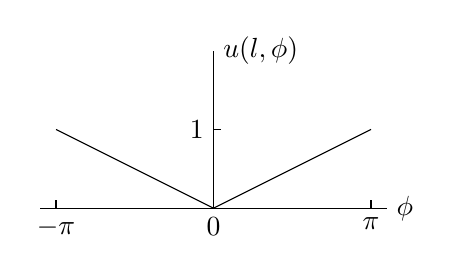
\begin{tikzpicture}
\draw(-2.2,0)--(2.2,0)node[right]{$\phi$};
\draw(0,0)node[below]{$0$}--(0,2)node[right]{$u(l,\phi)$};
\draw(-2,1)--(0,0)--(2,1);
\draw(-2,0)node[below]{$-\pi$}--++(0,0.1);
\draw(2,0)node[below]{$\pi$}--++(0,0.1);
\draw(0,1)node[left]{$1$}--++(0.1,0);
\end{tikzpicture}
\end{subfigure}%
\begin{subfigure}{0.5\textwidth}
\centering
\begin{tikzpicture}
\node[anchor=south west,inner sep=0] (image) at (0,0){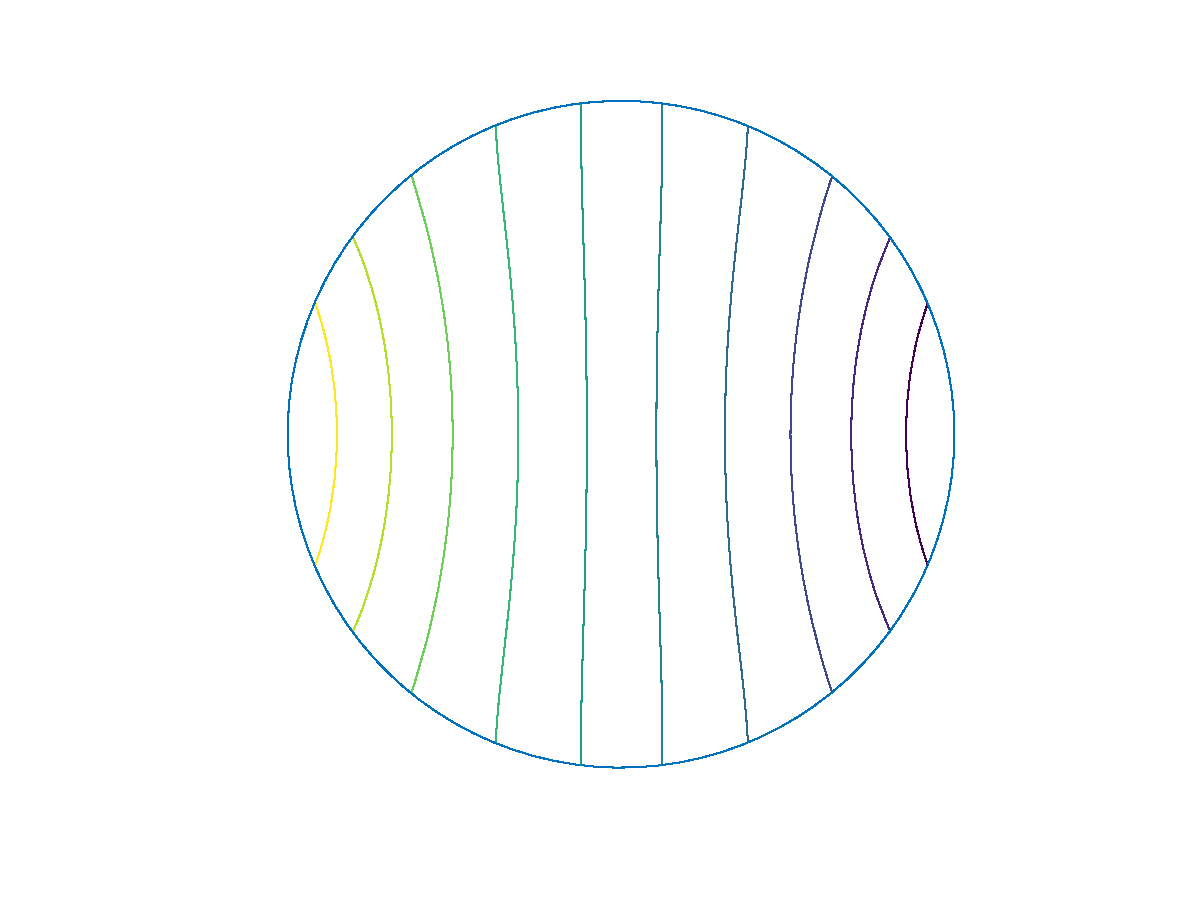
\includegraphics[width=4cm]{kcontour-inc}};
\begin{scope}[x={(image.south east)},y={(image.north west)}]
%  \draw[step=0.1] (0,0) grid (1,1);
%\draw[step=0.01,thin,gray] (0,0) grid (1,1);
\draw(0.85,0.75)node[rotate=45,font=\footnotesize]{$0.1$};
\draw(0.8,0.85)node[rotate=50,font=\footnotesize]{$0.2$};
\draw(0.72,0.95)node[rotate=60,font=\footnotesize]{$0.3$};
\draw(0.6,1)node[rotate=75,font=\footnotesize]{$0.4$};
%
\draw(0.2,0.75)node[shift={(-0.08,0.02)},rotate=-45,font=\footnotesize]{$u=0.9$};
\draw(0.2,0.85)node[rotate=-50,font=\footnotesize]{$0.8$};
\draw(0.28,0.95)node[rotate=-60,font=\footnotesize]{$0.7$};
\draw(0.4,1)node[rotate=-75,font=\footnotesize]{$0.6$};
\draw(0.15,0.5)--(0.9,0.5)node[right]{$x$};
\draw (0.52,0.11)--(0.52,0.92);
\draw(0.52,0.92)--++(0,0.1)node[above]{$y$};
\draw(0.212,0.5)node[ocirc]{};
\draw(0.82,0.5)node[ocirc]{};
    \end{scope}
\end{tikzpicture}
\end{subfigure}%
\caption{سرحدی مخفی قوہ (مثال \حوالہ{مثال_مخفی_ڈرشلے_الف})}
\label{شکل_مثال_مخفی_ڈرشلے_الف}
\end{figure}

\انتہا{مثال}
%=========================

\حصہء{سوالات}

%=======================
\ابتدا{سوال}\quad 
مساوات \حوالہ{مساوات_مخفی_معمہ_پ} کی تصدیق کریں۔
\انتہا{سوال}
%=========================
\ابتدا{سوال}\quad
دکھائیں کہ مساوات \حوالہ{مساوات_مخفی_معمہ_چ} کا ہر جزو قرص \عددی{r^2<R^2} میں ہارمونی تفاعل ہے۔
\انتہا{سوال}
%========================
مساوات \حوالہ{مساوات_مخفی_معمہ_چ} استعمال کرتے ہوئے سوال \حوالہ{سوال_مخفی_ڈرشلے_ب} تا سوال \حوالہ{سوال_مخفی_ڈرشلے_الف} میں اکائی قرص \عددی{r<1} میں مخفی قوہ \عددی{u(r,\theta)} تلاش کریں۔قرص کی سرحد پر مخفی قوہ \عددی{u(1,\theta)} ہے۔تسلسل کے چند ابتدائی اجزاء کے مجموعہ سے \عددی{u} کی قیمت حاصل کرتے ہوئے ہم قوہ خطوط کا ترسیم کھینچیں۔

%=============================  
\ابتدا{سوال}\شناخت{سوال_مخفی_ڈرشلے_الف}\quad
$u(1,\theta)=\sin\theta$\\
جواب:\quad
$u=r\sin\theta$
\انتہا{سوال}
%=======================
\ابتدا{سوال}\quad
$u(1,\theta)=1-\cos\theta$\\
جواب:\quad
$u=1-r\cos\theta$
\انتہا{سوال}
%=======================
\ابتدا{سوال}\quad
$u(1,\theta)=\sin 3\theta$\\
جواب:\quad
$u=r^3\sin 3\theta$
\انتہا{سوال}
%=======================
\ابتدا{سوال}\quad
$u(1,\theta)=\cos 2\theta-\cos 4\theta$\\
جواب:\quad
$u=r^2\cos 2\theta-r^4\cos 4\theta$
\انتہا{سوال}
%=======================
\ابتدا{سوال}\quad
$u(1,\theta)=4\sin^3 \theta$\\
جواب:\quad
$3r\sin\theta-r^3\sin3\theta$
\انتہا{سوال}
%======================
\ابتدا{سوال}\شناخت{سوال_مخفی_درکار_الف}\quad
$u(1,\theta)=\theta$\\
جواب:\quad
$\pi-2r\sin\theta-r^2\sin 2\theta-\tfrac{2r^3}{3}\sin 3\theta-\tfrac{r^4}{2}\sin4\theta-\cdots$
\انتہا{سوال}
%=======================
\ابتدا{سوال}\quad
\عددی{0<\theta<\pi} پر \عددی{u(1,\theta)=1} ہے جبکہ اس وقفہ کے علاوہ \عددی{u(1,\theta)=0} ہے۔\\
جواب:\quad
$\tfrac{1}{2}+\tfrac{2}{\pi}(r\sin \theta+\tfrac{r^3}{3}\sin 3\theta+\tfrac{r^5}{5}\sin 5\theta+\cdots)$
\انتہا{سوال}
%=======================
\ابتدا{سوال}\quad
\عددی{-\tfrac{\pi}{2}<\theta<\tfrac{\pi}{2}} پر \عددی{u(1,\theta)=\theta} ہے جبکہ \عددی{\tfrac{\pi}{2}<\theta<\tfrac{3\pi}{2}} پر 
\عددی{u(1,\theta)=\pi-\theta} ہے۔\\
جواب:\quad
$\tfrac{4}{\pi}(r\sin\theta-\tfrac{r^3}{9}\sin 3\theta+\tfrac{r^5}{25}\sin5\theta-\tfrac{r^7}{49}\sin7\theta\cdots)$
\انتہا{سوال}
%=======================
\ابتدا{سوال}\quad
\عددی{-\pi<\theta<-\tfrac{\pi}{2}} پر \عددی{u(1,\theta)=-\tfrac{\pi}{2}} ہے، \عددی{-\tfrac{\pi}{2}<\theta<\tfrac{\pi}{2}} پر 
\عددی{u(1,\theta)=\theta} ہے اور \عددی{\tfrac{\pi}{2}<\theta<\pi} پر \عددی{u(1,\theta)=\tfrac{\pi}{2}} ہے۔\\
جواب:\quad
$(1+\tfrac{2}{\pi})r\sin\theta-\tfrac{r^2}{2}\sin2\theta+(\tfrac{1}{3}-\tfrac{2}{9\pi})r^3\sin3\theta-\tfrac{r^4}{4}\sin4\theta\cdots$
\انتہا{سوال}
%=======================
\ابتدا{سوال}\شناخت{سوال_مخفی_ڈرشلے_ب}\quad
\عددی{0<\theta<\tfrac{\pi}{2}}  پر \عددی{u(1,\theta)=1} ہے، \عددی{\tfrac{\pi}{2}<\theta<\pi} پر \عددی{u(1,\theta)=-1} ہے جبکہ باقی تمام \عددی{\theta} پر \عددی{u(1,\theta)=0} ہے۔\\
جواب:\quad
$\tfrac{2}{\pi}(r\cos\theta+r^2\sin2\theta-\tfrac{r^3}{3}\cos3\theta+\tfrac{r^5}{5}\cos 5\theta\cdots )$
\انتہا{سوال}
%=========================
\ابتدا{سوال}\quad
مساوات \حوالہ{مساوات_ٹیلر_لوگارتھمی_کسر} استعمال کرتے ہوئے دکھائیں کہ  سوال \حوالہ{سوال_مخفی_ڈرشلے_ب} کے نتیجہ کو  درج ذیل لکھا جا سکتا ہے۔
\begin{align*}
u(r,\theta)=\frac{1}{\pi}\Ln\frac{(1+iz)(1+z^2)}{(1-iz)(1-z^2)}\text{خیالی}
\end{align*}
\انتہا{سوال}
%=====================
\ابتدا{سوال}\quad 
دکھائیں کہ سوال \حوالہ{سوال_مخفی_درکار_الف} کی مخفی قوہ کو \عددی{u(r,\theta)=2\Ln (1+z)\text{خیالی}} لکھا جا سکتا ہے۔
\انتہا{سوال}
%=============================
\ابتدا{سوال}\شناخت{سوال_مخفی_درکار_ب}\quad
مساوات \حوالہ{مساوات_مخفی_معمہ_چ} استعمال کرتے ہوئے دکھائیں کہ  اکائی قرص \عددی{r<1}، جس کا سرحدی مخفی قوہ 
\begin{align*}
u(1,\theta)=
\begin{cases}
-1&-\pi<\theta<0\\
\phantom{-}1&\phantom{-1}0<\theta<\pi
\end{cases}
\end{align*}
ہو،  کے اندر مخفی قوہ \عددی{u(r,\theta)} درج ذیل ہو گا۔
\begin{align*}
u(r,\theta)=\frac{4}{\pi}(r\sin\theta+\tfrac{r^3}{3}\sin3\theta+\tfrac{r^5}{5}\sin 5\theta+\cdots)
\end{align*}
اس تسلسل کے چند ابتدائی اجزاء استعمال کرتے ہوئے \عددی{u} کی قیمتیں حاصل کر کے چند ہم قوہ خطوط ترسیم کریں۔ قوت کی لکیروں (قائمہ الزاویہ خطوط) کو  ترسیم کر کے ان کا شکل \حوالہ{شکل_سوال_مخفی_درکار_ب} کے ساتھ موازنہ کریں۔
\begin{figure}
\centering

\begin{tikzpicture}[x={(0,0cm)},y={(1cm,0cm)},
    z={(0cm,1cm)}]
\begin{scope}[rotate=90]
\pgfmathsetmacro{\r}{1.5}
\foreach \phi in {-72,-54,...,72}{\draw[] ({0},{0},\r)
                \foreach \theta in {5,10,...,180}{--({\r*sin(\phi)*cos(\theta)},{\r*sin(\phi)*sin(\theta)},{\r*cos(\theta)})};}
\foreach \phi/\u in {-18/-0.2,-52/-0.6,54/0.6,18/0.2}{\draw({\r*sin(\phi)*cos(90)},{\r*sin(\phi)*sin(90)},{\r*cos(90)})node[fill=white,font=\tiny]{$\u$};}
\draw(0,0,\r)node[ocirc]{};
\draw(0,0,-\r)node[ocirc]{}--++(0,0,-0.4)node[right]{$x$};
\draw(0,1.05*\r,0)--++(0,0.4,0)node[left]{$y$};
\draw(0,1*\r,-0.525*\r)node[rotate=-20]{$u=1$};
\draw(0,-1.02*\r,0)node[]{$u=-1$};
\end{scope}
\end{tikzpicture}
\caption{شکل برائے سوال \حوالہ{سوال_مخفی_درکار_ب}}
\label{شکل_سوال_مخفی_درکار_ب}
\end{figure}
%

\انتہا{سوال}
%=============================
\ابتدا{سوال}\شناخت{سوال_مخفی_درکار_پ}\quad
مساوات \حوالہ{مساوات_ٹیلر_لوگارتھمی_کسر} استعمال کرتے ہوئے  دکھائیں کہ سوال \حوالہ{سوال_مخفی_درکار_ب} کے نتیجہ کو درج ذیل لکھا جا سکتا ہے۔
\begin{align*}
u(r,\theta)=\frac{2}{\pi}\Ln\frac{1+z}{1-z}\text{خیالی}=\frac{2}{\pi}(\,\,\phase{1+z}-\phase{1-z}\,\,)
\end{align*}
\انتہا{سوال}
%======================
\ابتدا{سوال}\quad
جیومیٹری کے ایک بنیادی مسئلے کو سوال \حوالہ{سوال_مخفی_درکار_پ} کے نتیجے پر لاگو کرتے ہوئے دکھائیں کہ سوال \حوالہ{سوال_مخفی_درکار_ب} میں \عددی{u=\text{مستقل}} دائری قوس ہیں۔
\انتہا{سوال}
%=========================
\ابتدا{سوال}\شناخت{سوال_مخفی_درکار_ت}\quad
دکھائیں کہ بالائی نصف مستوی \عددی{v>0} میں درج ذیل ہارمونی ہے اور وقفہ \عددی{-1<u<1} پر اس کی قیمت \عددی{-1} جبکہ باقی \عددی{u} محور  پر اس کی قیمت \عددی{+1} ہے۔ 
\begin{align*}
H=1+\frac{2}{\pi}\Ln\frac{w+1}{w-1}\text{خیالی}\quad\quad \quad (w=u+iv)
\end{align*}
\انتہا{سوال}
%===========================
\ابتدا{سوال}\quad
دکھائیں کہ وہ خطی کسری تبادل جو \عددی{w_1=-1}، \عددی{w_2=0}، \عددی{w_3=1} کو بالترتیب \عددی{z_1=-1}، \عددی{z_2=-i}، \عددی{z_3=1}  پر نقش کرتا ہو
\begin{align*}
z=\frac{w-i}{-iw+1}
\end{align*}
ہے۔اس کا الٹ تبادل \عددی{w=w(z)} تلاش کرتے ہوئے سوال \حوالہ{سوال_مخفی_درکار_ت} میں دیے گئے \عددی{H} میں پر کرتے ہوئے دکھائیں کہ حاصل ہارمونی تفاعل سوال \حوالہ{سوال_مخفی_درکار_پ} کا ہارمونی تفاعل ہے۔
\انتہا{سوال}
%===========================
\ابتدا{سوال}\quad
مسئلہ \حوالہ{مسئلہ_مخفی_ہارمونی_تفاعل_کے_جزوی_تفرق} کو پوسوں کلیہ تکمل مساوات \حوالہ{مساوات_مخفی_معمہ_ٹ} سے اخذ کریں۔
\انتہا{سوال}
%===============================


